\documentclass[11pt,twocolumn]{article}
\usepackage[margin=1in]{geometry}
\usepackage{times}
\usepackage{booktabs}
\usepackage{xcolor}
\usepackage{microtype}
\usepackage{amsmath}
\usepackage{hyperref}
\usepackage[authoryear]{natbib}
\usepackage{graphicx}
\usepackage{longtable}
\usepackage[affil-it]{authblk} 

% Visible placeholder boxes
\newcommand{\fillp}[2]{%
  \par\noindent
  \colorbox{yellow!60}{\parbox{\linewidth-2\fboxsep}{%
    \textbf{\textcolor{red}{[FILL -- #1:}} \textit{#2}\textbf{]}%
  }}%
  \par
}
\newcommand{\fillbox}[2]{%
  \colorbox{yellow!60}{%
    \textbf{\textcolor{red}{[#1: #2]}}%
  }%
}

\title{\textbf{Fairness and Proxy Bias in Occupation Prediction:}\\
Scaling, Masking, and Mechanistic Attribution across Model Families}

\author{Usukhbayar Purevdorj}
\author{Yitong Kong}
\author{Kirill Kamakaev}
\author{Giulio Zhu}
\author{Kian Makela}
\author{Ambrose Yang}

\affil{University College London --- COMP0087 \\
\texttt{\{usukhbayar.purevdorj.25, yitong.kong.25, kirill.kamakaev.22, giulio.zhu.22, kian.makela.25, zhuohan.yang.25\}@ucl.ac.uk} \\
Code: \url{https://github.com/usukhbayarp/comp0087-fairness-occupation-prediction}}
\date{}

\begin{document}
\maketitle

% ── ABSTRACT ────────────────────────────────────────────────────
\begin{abstract}
We investigate gender bias and proxy feature encoding in occupation
prediction models trained on the Bias-in-Bios dataset.
Our study spans two dimensions: \emph{model capacity}, comparing
Pythia generative models (160M--1.4B parameters) across zero-shot,
few-shot, and fine-tuned regimes, and \emph{model architecture},
contrasting encoder-based classifiers (DistilBERT, RoBERTa) against
generative models of comparable performance.
We evaluate both task performance (Macro-F1) and gender fairness
(Equalized Odds gap, Demographic Parity) under masked and unmasked
conditions, and diagnose bias mechanisms through Integrated Gradients
attribution validated by top-$K$ token erasure.
Our main findings: (1) fine-tuned models substantially outperform
zero/few-shot baselines in both performance and fairness;
(2) larger models are not inherently fairer---zero-shot bias
\emph{increases} with scale; (3) gender-token masking reduces bias for some professions but produces backfire effects for others, suggesting that implicit proxy signals survive removal of explicit gender tokens; (4) explicit gender tokens are not the primary
drivers of bias---they appear with weights 100$\times$ smaller than
dominant profession tokens, while indirect contextual signals carry
the latent gender signal; and (5) proxy bias is model-dependent, the same profession 
can be stable under one model and unstable under another, 
though the precise cause (architecture, pre-training, or scale) 
cannot be isolated from this comparison alone.
\end{abstract}

% ── 1. INTRODUCTION ─────────────────────────────────────────────
\section{Introduction}

Occupation prediction from biographical text exposes persistent gender
stereotypes: models trained on real-world career data reliably
associate professions such as \emph{nurse} or \emph{dietitian} with
female-typical language patterns, and \emph{surgeon} or
\emph{software engineer} with male-typical ones. \citet{de-arteaga-etal-2019-bias} demonstrated on the Bias-in-Bios dataset
that scrubbing explicit gender signals does not eliminate these
disparities---implicit proxy features survive.

This paper addresses three open questions: how does model
\emph{capacity} interact with fairness; how does model
\emph{architecture} shape which proxy features are learned; and what
are those features precisely.

\paragraph{Contributions.}
(1) A scaling study across Pythia (160M--1.4B) in zero-shot, few-shot,
and fine-tuned regimes;
(2) a cross-model comparison of encoder baselines (DistilBERT, RoBERTa)
against the best Pythia configuration;
(3) an Integrated Gradients proxy audit by profession and gender group,
validated via top-$K$ token erasure faithfulness testing;
(4) a paired masked/unmasked evaluation measuring the effect of
gender-token scrubbing on both task performance and fairness metrics;
(5) a cross-model proxy stability analysis comparing attribution
patterns across encoder models.
To our knowledge, no prior work on the Bias-in-Bios occupation
prediction task provides token-level attribution analysis stratified
by both profession and gender, nor compares proxy stability across
encoder models on this dataset.

\paragraph{Key Findings.}
(1) Fine-tuned models substantially outperform zero/few-shot baselines
in both performance and fairness \citep{bommasani2021opportunities};
(2) zero-shot bias \emph{increases} with model scale, with the
Equalized Odds gap growing from ${\sim}0.09$ at 160M to ${\sim}0.21$
at 1.4B parameters;
(3) gender-token masking reduces bias inconsistently and produces
backfire effects for some professions, consistent with
\citet{romanov-etal-2019-whats};
(4) bias operates primarily through indirect contextual signals;
explicit gender tokens appear with weights over 100$\times$ smaller
than dominant profession tokens \citep{de-arteaga-etal-2019-bias};
(5) proxy stability is model-dependent---the same profession can be
stable under one model and unstable under another.
We do not claim that these findings generalise beyond the
Bias-in-Bios setting.

% ── 2. RELATED WORK ─────────────────────────────────────────────
\section{Related Work}

\textbf{Bias in occupation prediction.}
\citet{de-arteaga-etal-2019-bias} introduced Bias-in-Bios and showed that
classifiers exhibit gender disparities even after pronoun scrubbing.
\citet{romanov-etal-2019-whats} analysed limits of de-biasing through scrubbing.
We extend these findings by identifying and quantifying specific proxy
tokens through gradient-based attribution.

\textbf{Fairness metrics.}
\citet{hardt2016equality} formalised Equalized Odds; \citet{dwork2012fairness} introduced demographic parity. We evaluate both using a one-vs-rest
multiclass extension macro-averaged over occupations.

\textbf{Attribution methods.}
\citet{sundararajan2017axiomatic} introduced Integrated Gradients satisfying
completeness and sensitivity axioms. Attribution methods have been
applied to gender bias in coreference \citep{attanasio2022entropy} but
their systematic use in occupation classification is limited.
Critically, no prior work on the Bias-in-Bios occupation prediction 
task provides token-level proxy word tables with quantified attribution 
weights, nor examines how those weights shift under gender masking.

\textbf{Model scaling and fairness.}
\citet{bommasani2021opportunities} discusses risks of foundation models including
bias amplification. Our scaling study provides empirical evidence that
zero-shot bias increases with model size in the Pythia family.

\textbf{Gender masking.}
\citet{lu-etal-2020-gender} study counterfactual data augmentation for gender
bias. Unlike prior work, we measure not only the effect of masking on fairness metrics but also on token-level attribution patterns —
providing the first internal view of how occupation
prediction models redistribute feature importance when
gender signals are removed.

% ── 3. DATASET ──────────────────────────────────────────────────
\section{Dataset and Preprocessing}

\subsection{Bias-in-Bios}
We use the Bias-in-Bios dataset \citep{de-arteaga-etal-2019-bias}, accessed
via HuggingFace Datasets (\texttt{LabHC/bias\_in\_bios}). Bias-in-Bios has become a standard benchmark in the NLP fairness community for studying occupational gender stereotypes \citep{de-arteaga-etal-2019-bias, romanov-etal-2019-whats}. Each example contains a biography (\texttt{hard\_text}), an integer profession label, and a binary gender attribute (0\,$\to$\,M,
1\,$\to$\,F, provided by the dataset and inferred from 
pronoun usage in the biography text by the original authors).
We restrict to the \textbf{top 20 most frequent occupations} computed
from the training split, filtering out all other examples.
The task is to predict a biography's occupation label---one of these
20 classes---from its free-text content alone; gender is used only
as a post-hoc evaluation attribute and never as a model input.

\begin{table}[h]
\centering\small
\begin{tabular}{lrrr}
\toprule
\textbf{Split} & \textbf{Total} & \textbf{Female} & \textbf{Male} \\
\midrule
Train & 248,141 & 46.16\% & 53.84\% \\
Dev   &  38,198 & 46.16\% & 53.84\% \\
Test  &  95,468 & 46.17\% & 53.83\% \\
\midrule
\textbf{Total} & \textbf{381,807} & 46.16\% & 53.84\% \\
\bottomrule
\end{tabular}
\caption{Dataset split sizes and gender distribution. The near-identical
F\% across splits (range: 0.01\%, i.e.\ approximately 46.2\% female
in each) indicates the original dataset was stratified by gender
when partitioned.}
\end{table}

Table~\ref{tab:professions} shows the per-profession counts and gender
distribution in the training split. Several occupations exhibit strong
gender skew: \emph{dietitian} (92.9\% F), \emph{nurse} (90.8\% F),
and \emph{model} (82.7\% F) are heavily female-dominated, while
\emph{surgeon} (14.8\% F), \emph{software engineer} (15.8\% F), and
\emph{composer} (16.4\% F) are heavily male-dominated.

\begin{table}[h]
\centering\small
\setlength{\tabcolsep}{4pt}
\begin{tabular}{lrr}
\toprule
\textbf{Profession} & \textbf{N (train)} & \textbf{F\%} \\
\midrule
professor         & 76,748 & 45.1 \\
physician         & 26,648 & 49.4 \\
attorney          & 21,169 & 38.3 \\
photographer      & 15,773 & 35.7 \\
journalist        & 12,960 & 49.5 \\
nurse             & 12,316 & 90.8 \\
psychologist      & 11,945 & 62.1 \\
teacher           & 10,531 & 60.2 \\
dentist           &  9,479 & 35.3 \\
surgeon           &  8,829 & 14.8 \\
architect         &  6,568 & 23.7 \\
painter           &  5,025 & 45.7 \\
model             &  4,867 & 82.7 \\
filmmaker         &  4,545 & 32.9 \\
poet              &  4,558 & 49.0 \\
software engineer &  4,492 & 15.8 \\
composer          &  3,637 & 16.4 \\
accountant        &  3,660 & 36.7 \\
dietitian         &  2,567 & 92.9 \\
comedian          &  1,824 & 21.1 \\
\bottomrule
\end{tabular}
\caption{Per-profession training counts and F\% (M\%\,=\,100\,$-$\,F\%).
Distribution is consistent across all splits.}
\label{tab:professions}
\end{table}

\subsection{Evaluation Subset}
All models are evaluated on a canonical \textbf{3,000-sample test
subset}, stratified by profession proportionally to each profession's
frequency in the full test set, and sampled from the 95,468-example
test split. A shared canonical ID list ensures comparability across
all models and regimes.

The 3,000-sample subset was chosen to balance statistical
representativeness against two computational constraints: (1) the
latency of zero-shot and few-shot inference over the full 95K test
split, and (2) the cost of running Integrated Gradients attribution
across four conditions (two encoder models $\times$ two masking
conditions), each requiring a separate forward pass per example. Per-profession sample sizes range
from 932 (professor) to 27 (comedian); results for low-frequency
professions should be interpreted with caution given the small
sample sizes.

\subsection{Gender Masking}
Two conditions: \textbf{Unmasked} (original text) and
\textbf{Masked} (explicit gender tokens replaced with
\texttt{[MASK]} for DistilBERT and \texttt{<mask>} for RoBERTa,
matching each model's native mask token), applied via exact
case-insensitive word-boundary regex matching
(\texttt{\textbackslash b...\textbackslash b}).
Three categories of tokens are masked:
(1)~\textbf{Pronouns and possessives}: \emph{he, she, his, her, him,
hers, himself, herself};
(2)~\textbf{Titles and honorifics}: \emph{mr, mr., mister, mrs, mrs.,
miss, ms, ms., madam, madame, ma'am, sir, lady, lord, dame};
(3)~\textbf{Gendered nouns} (35 terms including \emph{father, mother,
husband, wife, son, daughter, brother, sister, actor, actress,
businessman, businesswoman, waiter, waitress}, and others).
Masking is disabled by default and enabled per experiment.
Name masking was not applied for two reasons: (1) any general-purpose
name-masking rule introduces uncontrolled noise through false positives
and false negatives; and (2) names carry biographical content beyond
gender---masking them would conflate the removal of gender signals with
a broader loss of biographical information, undermining the internal
validity of the masked/unmasked comparison.

% ── 4. METHODS ──────────────────────────────────────────────────
\section{Methods}

\subsection{Pythia: Zero-shot and Few-shot}
We evaluate Pythia \citep{biderman2023pythia} at 160M, 410M, and 1.4B parameters under two inference regimes: zero-shot and few-shot, with and without gender masking applied to the input biography.

\medskip

\noindent
\textbf{Zero-shot}: biography + candidate list, no examples.
\textbf{Few-shot}: $K=4$ exemplars pairs prepended to prompt.

\medskip

Since Pythia is a causal language model rather than a classifier, occupation prediction is framed as a \textit{candidate scoring} problem. Given a prompt $p$ and a set of candidate label strings $\mathcal{C} = \{c_1, \ldots, c_N\}$, we score each candidate by computing the joint log-probability of its token sequence conditioned on the prompt via the chain rule:
\begin{equation} \log P(c_k \mid p) = \sum_{t=1}^{|c_k|} \log P!\left(c_k^{(t)} \mid p, c_k^{(1)}, \ldots, c_k^{(t-1)}\right) \end{equation}
Each candidate is appended to the prompt token sequence and the log-probability of each candidate token is extracted at its absolute position in the combined sequence. The predicted label is then:
\begin{equation} 
    \hat{y} = \arg\max_{c_k \in \mathcal{C}} \log P(c_k \mid p) 
\end{equation}
To produce a confidence proxy across candidates, we apply a softmax over the raw log-probability scores:
\begin{equation} 
    \mathrm{conf}_k = \frac{\exp\!\left(\log P(c_k \mid p)\right)}{\displaystyle\sum_{j} \exp\!\left(\log P(c_j \mid p)\right)}
\end{equation}
We report \textbf{conf} as the softmax probability assigned to the predicted label $\hat{y}$, reflecting the model's relative preference among candidates. We additionally report \textbf{score} as the log of the confidence proxy:
\begin{equation}
    \mathrm{score} = \log(\mathrm{conf} + 10^{-12})
\end{equation}
where $10^{-12}$ ensures numerical stability when confidence approaches zero. All predictions are saved in a shared JSONL format recording the true label, predicted label, gender, model size, inference regime, and both metrics.

\subsection{Pythia: Supervised Fine-tuning}
Pythia is treated as a sequence classifier with a classification head over the final hidden state. Training uses the HuggingFace Trainer, with the best checkpoint selected by dev Macro-F1. By default, unless full fine-tuning is explicitly enabled, LoRA \citep{hu2022lora} is applied to the attention \texttt{query\_key\_value} projections in every transformer layer, with rank $r=16$, $\alpha=32$, and dropout $0.1$. The default setup uses a learning rate of $2\times10^{-5}$, batch size $16$, $3$ epochs, linear decay with warmup ratio $0.06$, weight decay $0.01$, and maximum sequence length $256$. For larger models such as Pythia-1.4B, optional 4-bit quantisation (QLoRA) can be used to reduce memory requirements.

\subsection{Encoder Baselines: DistilBERT and RoBERTa}
To provide supervised baselines from a distinct architectural
family, DistilBERT \citep{sanh2019distilbert} (66M parameters) and RoBERTa-base \citep{liu2019roberta} (125M parameters) are fine-tuned as sequence classi-
fiers with a linear classification head over the encoder
representation. Inputs are tokenised
with the model specific tokeniser and truncated to a maximum length
of 256 tokens. Training is performed for 3 epochs with a learning
rate of $2\times10^{-5}$ and batch size 16 (evaluation batch size 32).
Dynamic padding is applied and the best checkpoint is selected based
on Macro-F1, accounting for class imbalance. The same
pipeline is used for both masked and unmasked conditions with a shared
label mapping. Evaluation is performed on the shared 3,000-example test
subset, ensuring direct comparability with the generative models.

%\subsection{Fairness Evaluation}
%Metrics: Macro-F1, Accuracy, Demographic Parity (DP) gap, and
%Equalized Odds (EO) gap $= \max(\overline{\Delta\text{TPR}}, \overline{\Delta\text{FPR}})$,
%where $\overline{\Delta\text{TPR}}$ and $\overline{\Delta\text{FPR}}$ are
%the macro-averaged TPR and FPR gaps respectively across the 20
%one-vs-rest occupation classifiers.

\subsection{Evaluation Metrics}
\label{sec:evaluation}

We evaluate models on both task performance and fairness. Let $Y$ represent the true occupation label, $\hat{Y}$ the predicted label, $A \in \{M, F\}$ the binary gender attribute, and $\mathcal{C}$ the set of 20 occupation classes. 

\textbf{Task Performance:} We report overall Accuracy and Macro-F1 score to account for the heavy class imbalance present in the dataset.

\textbf{Fairness Metrics:} We measure gender disparities using one-vs-rest multiclass extensions of Demographic Parity (DP) and Equalized Odds (EO), macro-averaged across all occupations. 

Demographic Parity requires the prediction to be independent of the sensitive attribute. We compute the macro-averaged DP gap as the absolute difference in positive prediction rates between genders for each class:

\vspace{-1em}

\begin{align*}
\Delta \text{DP} = \frac{1}{|\mathcal{C}|} \sum_{c \in \mathcal{C}} \Big| & P(\hat{Y} = c \mid A = M) \\
&- P(\hat{Y} = c \mid A = F) \Big|
\end{align*}

Equalized Odds requires the prediction to be conditionally independent of the sensitive attribute given the true label. To compute the EO gap, we first calculate the macro-averaged True Positive Rate (TPR) gap and False Positive Rate (FPR) gap:

\vspace{-1em}

\begin{align*}
\Delta \text{TPR} = \frac{1}{|\mathcal{C}|} \sum_{c \in \mathcal{C}} \Big| & P(\hat{Y} = c \mid Y = c, A = M) \\
&- P(\hat{Y} = c \mid Y = c, A = F) \Big|
\end{align*}

\vspace{-1.6em}

\begin{align*}
\Delta \text{FPR} = \frac{1}{|\mathcal{C}|} \sum_{c \in \mathcal{C}} \Big| & P(\hat{Y} = c \mid Y \neq c, A = M) \\
&- P(\hat{Y} = c \mid Y \neq c, A = F) \Big|
\end{align*}

The final Equalized Odds gap is defined as the maximum of these two macro-averaged disparities:
$$ \text{EO Gap} = \max(\Delta \text{TPR}, \Delta \text{FPR}) $$

\subsection{Proxy Bias Attribution}
Integrated Gradients \citep{sundararajan2017axiomatic} is applied to the
two fine-tuned encoder models, with attribution computed toward the
\emph{predicted} class index.
Attributions are computed using \textbf{32 interpolation steps} and a
\textbf{zero-embedding baseline}.
Token-level scores are obtained by \textbf{summing} attribution values
across the embedding dimension for each token position.
Subword tokens are merged to word level before top-$K$ selection:
BERT-style \texttt{\#\#} continuation pieces and whitespace-prefixed tokens (RoBERTa's byte-pair encoding marks word boundaries with a special prefix character) are handled separately, with scores summed
across pieces.
Only tokens with \textbf{positive} attribution scores and minimum
length of 2 characters are retained.
Maximum sequence length is \textbf{256 tokens}.

The pipeline operates in two stages with distinct $K$ values.
\textbf{Stage 1 --- per-example extraction} ($K_1\!=\!5$): the 5
highest-scoring positive tokens are retained per example.
\textbf{Stage 2 --- profession-level aggregation}: tokens appearing
across all examples for a profession are aggregated (minimum length
3, stopwords removed) to compute:
\begin{equation}
  \text{wscore}(t,p) = \text{count\_topk}(t,p) \times \overline{\text{attr}}(t,p)
\end{equation}
where $\text{count\_topk}(t,p)$ is the number of examples in which
token $t$ appears in the stage-1 top-5 for profession $p$, and
$\overline{\text{attr}}(t,p)$ is the mean attribution score.
Aggregation uses the model's \emph{predicted} label (not the true
label), consistent with attribution targeting the predicted class.

\textbf{Stability analysis.}
The masked vs.\ unmasked comparison takes the \textbf{top-10
aggregated tokens} per profession ($K_2\!=\!10$) and computes the
shared token ratio:
\begin{equation}
  r(p) = \frac{|\mathcal{T}_\text{sh}|}{
    |\mathcal{T}_\text{sh}|+|\mathcal{T}_\text{m}|+|\mathcal{T}_\text{u}|}
\end{equation}
where $\mathcal{T}_\text{sh}$, $\mathcal{T}_\text{m}$,
$\mathcal{T}_\text{u}$ are the sets of tokens shared, masked-only,
and unmasked-only respectively among the top-10.
Gender-conditioned proxy tables are produced identically, stratified
by profession and gender field.
$K_2 > K_1$ is appropriate because aggregation across many examples
yields a richer profession-level vocabulary than any single example
produces; $K_1$ limits per-example computation while $K_2$ captures
the most salient profession-level features.

\textbf{Faithfulness validation.}
To validate that the identified proxy tokens are causally load-bearing
rather than merely correlated with the prediction, we perform a
top-$K$ erasure faithfulness test: the top-5 attributed tokens are
masked in each example's text and the model is re-run to measure the
probability drop for the predicted class:
\begin{equation}
  \text{Faith}(x) = P(y \mid x) - P(y \mid x_{\text{erased}})
\end{equation}
A high faithfulness score indicates the attributed tokens causally influence the prediction.

% ── 5. EXPERIMENTAL SETUP ───────────────────────────────────────
\section{Experimental Setup}

\begin{table}[h]
\centering\small
\setlength{\tabcolsep}{4pt}
\begin{tabular}{llll}
\toprule
\textbf{Model} & \textbf{Type} & \textbf{Regime} & \textbf{Cond.} \\
\midrule
Pythia-160M & Gen. & zero-shot, few-shot, FT & M, U \\
Pythia-410M & Gen. & zero-shot, few-shot, FT & M, U \\
Pythia-1.4B & Gen. & zero-shot, few-shot, FT & M, U \\
DistilBERT  & Enc. & Fine-tuned           & M, U \\
RoBERTa     & Enc. & Fine-tuned           & M, U \\
\bottomrule
\end{tabular}
\caption{All model configurations. FT=fine-tuned; M=masked; U=unmasked.}
\end{table}

%All models output a shared JSONL format:
%\texttt{\{id, label\_true, label\_pred, gender, model, regime, conf\}}.
%A $\sim$4\% mismatch between stored and recomputed RoBERTa unmasked
%predictions introduces minor noise; as this mismatch is not
%concentrated in any specific profession, its effect is assumed to be
%approximately uniform across categories.

To systematically evaluate the drivers of proxy bias in occupation prediction, our experiments are structured around two primary axes: model capacity and model architecture. We compare the Pythia family of generative models at three distinct scales (160M, 410M, and 1.4B parameters) against established encoder-based baselines, specifically DistilBERT and RoBERTa.

We evaluate the Pythia models across three distinct learning regimes: zero-shot, few-shot, and supervised fine-tuning. This progression allows us to isolate how task-specific supervision impacts fairness and task performance compared to the raw, stereotypical associations embedded in the pre-trained foundation models. The encoder baselines are strictly evaluated in the fine-tuned regime to serve as a performance ceiling for the generative models.

Furthermore, to measure the specific impact of demographic scrubbing, every model configuration is evaluated under both Unmasked (original text) and Masked (explicit gender tokens replaced) conditions. This paired evaluation strategy establishes a clear baseline and isolates the effect of the masking intervention on both the Macro-F1 score and the Equalized Odds gap.

% ── 6. RESULTS ──────────────────────────────────────────────────
\section{Results and Discussion}

We evaluate our models across three dimensions: task performance
(§6.1), gender fairness (§6.2), and token-level proxy bias
mechanisms (§6.3).

\subsection{Task Performance}

\begin{table}[h]
\centering\small
\setlength{\tabcolsep}{5pt}
\begin{tabular}{llcc}
\toprule
\textbf{Model} & \textbf{C.} & \textbf{Acc.} & \textbf{F1} \\
\midrule
Pythia-160M FT & U & 0.082 & 0.020 \\
Pythia-160M FT & M & 0.124 & 0.023 \\
Pythia-410M FT & U & 0.579 & 0.320 \\
Pythia-410M FT & M & 0.575 & 0.328 \\
Pythia-1.4B FT & U & 0.876 & 0.849 \\
Pythia-1.4B FT & M & 0.875 & 0.847 \\
\midrule
DistilBERT FT  & U & 0.875 & 0.843 \\
DistilBERT FT  & M & 0.872 & 0.844 \\
RoBERTa FT     & U & 0.882 & 0.851 \\
RoBERTa FT     & M & 0.880 & 0.851 \\
\midrule
Pythia-160M zero-shot   & U & 0.405 & 0.230 \\
Pythia-160M zero-shot   & M & 0.400 & 0.223 \\
Pythia-160M few-shot    & U & 0.241 & 0.202 \\
Pythia-160M few-shot    & M & 0.249 & 0.206 \\
Pythia-410M zero-shot   & U & 0.536 & 0.557 \\
Pythia-410M zero-shot   & M & 0.533 & 0.553 \\
Pythia-410M few-shot    & U & 0.366 & 0.391 \\
Pythia-410M few-shot    & M & 0.363 & 0.389 \\
Pythia-1.4B zero-shot   & U & 0.658 & 0.567 \\
Pythia-1.4B zero-shot   & M & 0.659 & 0.568 \\
Pythia-1.4B few-shot    & U & 0.558 & 0.578 \\
Pythia-1.4B few-shot    & M & 0.558 & 0.577 \\
\bottomrule
\end{tabular}
\caption{Task performance. U=unmasked; M=masked.}
\end{table}

Fine-tuning yields a steep scaling benefit: Pythia-1.4B fine-tuned
achieves Macro-F1 of 0.849, matching encoder baselines (RoBERTa 0.851,
DistilBERT 0.843), while Pythia-160M remains effectively non-functional
after fine-tuning (F1\,$\approx$\,0.02, likely due to label-space
collapse under LoRA at insufficient model capacity).

Zero-shot performance scales with model size, improving from a macro-F1 of 0.23 (160M) to 0.57 (1.4B), where it plateaus. Masked variants at the same scale yield practically identical scores, suggesting masking has a negligible impact on predictive performance. Few-shot prompting is detrimental at smaller scales as the 160M and 410M models both perform worse under few-shot conditions (e.g., 410M drops from 0.557 to 0.391), indicating they lack the capacity to leverage in-context examples. At 1.4B, few-shot performance recovers to near zero-shot levels (0.578 vs. 0.567), implying a minimum capacity threshold must be met before few-shot prompting is beneficial.

Encoder models provide a strong supervised baseline across both
conditions. RoBERTa outperforms DistilBERT, achieving higher Macro-F1
(0.851 vs.\ 0.843) and accuracy, consistent with its larger capacity
and stronger pretraining. Unlike Pythia, encoder performance remains
stable, indicating that fine-tuned encoders effectively capture
task specific signals without requiring large scale scaling.

Masking has negligible impact on encoder performance, with
small changes observed for both DistilBERT
(0.843\,$\to$\,0.844) and RoBERTa (0.851\,$\to$\,0.851), while Pythia-1.4B is essentially unaffected
(0.849\,$\to$\,0.847). We next examine whether these performance differences translate to fairness disparities across gender groups.

\subsection{Fairness Results}
\label{sec:fairness}
\begin{table}[h]
\centering\small
\setlength{\tabcolsep}{4pt}
\begin{tabular}{llcccc}
\toprule
\textbf{Model} & \textbf{C.} & \textbf{EO} & \textbf{DP} & \textbf{TPR} & \textbf{FPR} \\
\midrule
\textbf{RoBERTa FT}     & \textbf{U} & \textbf{0.082} & \textbf{0.024} & \textbf{0.082} & \textbf{0.005} \\
RoBERTa FT              & M & 0.078 & 0.022 & 0.078 & 0.005 \\
\textbf{DistilBERT FT}  & \textbf{U} & \textbf{0.088} & \textbf{0.022} & \textbf{0.088} & \textbf{0.004} \\
DistilBERT FT           & M & 0.084 & 0.021 & 0.084 & 0.004 \\
\textbf{Pythia-1.4B FT} & \textbf{U} & \textbf{0.086} & \textbf{0.023} & \textbf{0.086} & \textbf{0.004} \\
Pythia-1.4B FT          & M & 0.080 & 0.022 & 0.080 & 0.003 \\
\textbf{Pythia-1.4B FS} & \textbf{U} & \textbf{0.121} & \textbf{0.031} & \textbf{0.121} & \textbf{0.016} \\
Pythia-1.4B FS          & M & 0.124 & 0.031 & 0.124 & 0.016 \\
\textbf{Pythia-1.4B 0s} & \textbf{U} & \textbf{0.210} & \textbf{0.029} & \textbf{0.210} & \textbf{0.019} \\
Pythia-1.4B 0s          & M & 0.210 & 0.029 & 0.210 & 0.019 \\
\textbf{Pythia-410m FT} & \textbf{U} & \textbf{0.085} & \textbf{0.012} & \textbf{0.085} & \textbf{0.006} \\
Pythia-410m FT          & M & 0.088 & 0.011 & 0.088 & 0.006 \\
\textbf{Pythia-410m FS} & \textbf{U} & \textbf{0.126} & \textbf{0.021} & \textbf{0.126} & \textbf{0.012} \\
Pythia-410m FS          & M & 0.128 & 0.020 & 0.128 & 0.011 \\
\textbf{Pythia-410m 0s} & \textbf{U} & \textbf{0.143} & \textbf{0.037} & \textbf{0.143} & \textbf{0.020} \\
Pythia-410m 0s          & M & 0.131 & 0.037 & 0.131 & 0.021 \\
\textbf{Pythia-160m FT} & \textbf{U} & \textbf{0.017} & \textbf{0.001} & \textbf{0.017} & \textbf{0.001} \\
Pythia-160m FT          & M & 0.003 & 0.002 & 0.003 & 0.002 \\
\textbf{Pythia-160m FS} & \textbf{U} & \textbf{0.080} & \textbf{0.012} & \textbf{0.080} & \textbf{0.007} \\
Pythia-160m FS          & M & 0.077 & 0.013 & 0.077 & 0.008 \\
\textbf{Pythia-160m 0s} & \textbf{U} & \textbf{0.092} & \textbf{0.027} & \textbf{0.092} & \textbf{0.025} \\
Pythia-160m 0s          & M & 0.092 & 0.027 & 0.092 & 0.024 \\
\bottomrule
\end{tabular}

\caption{Fairness metrics (EO = Equalized Odds gap, DP = Demographic Parity gap, TPR = True Positive Rate gap, FPR = False Positive Rate gap) for each model, both masked (M) and unmasked (U). Row label abbreviations: FT = fine-tuned; FS = few-shot; 0s = zero-shot.}
\end{table}

\begin{figure}[h!]
\centering
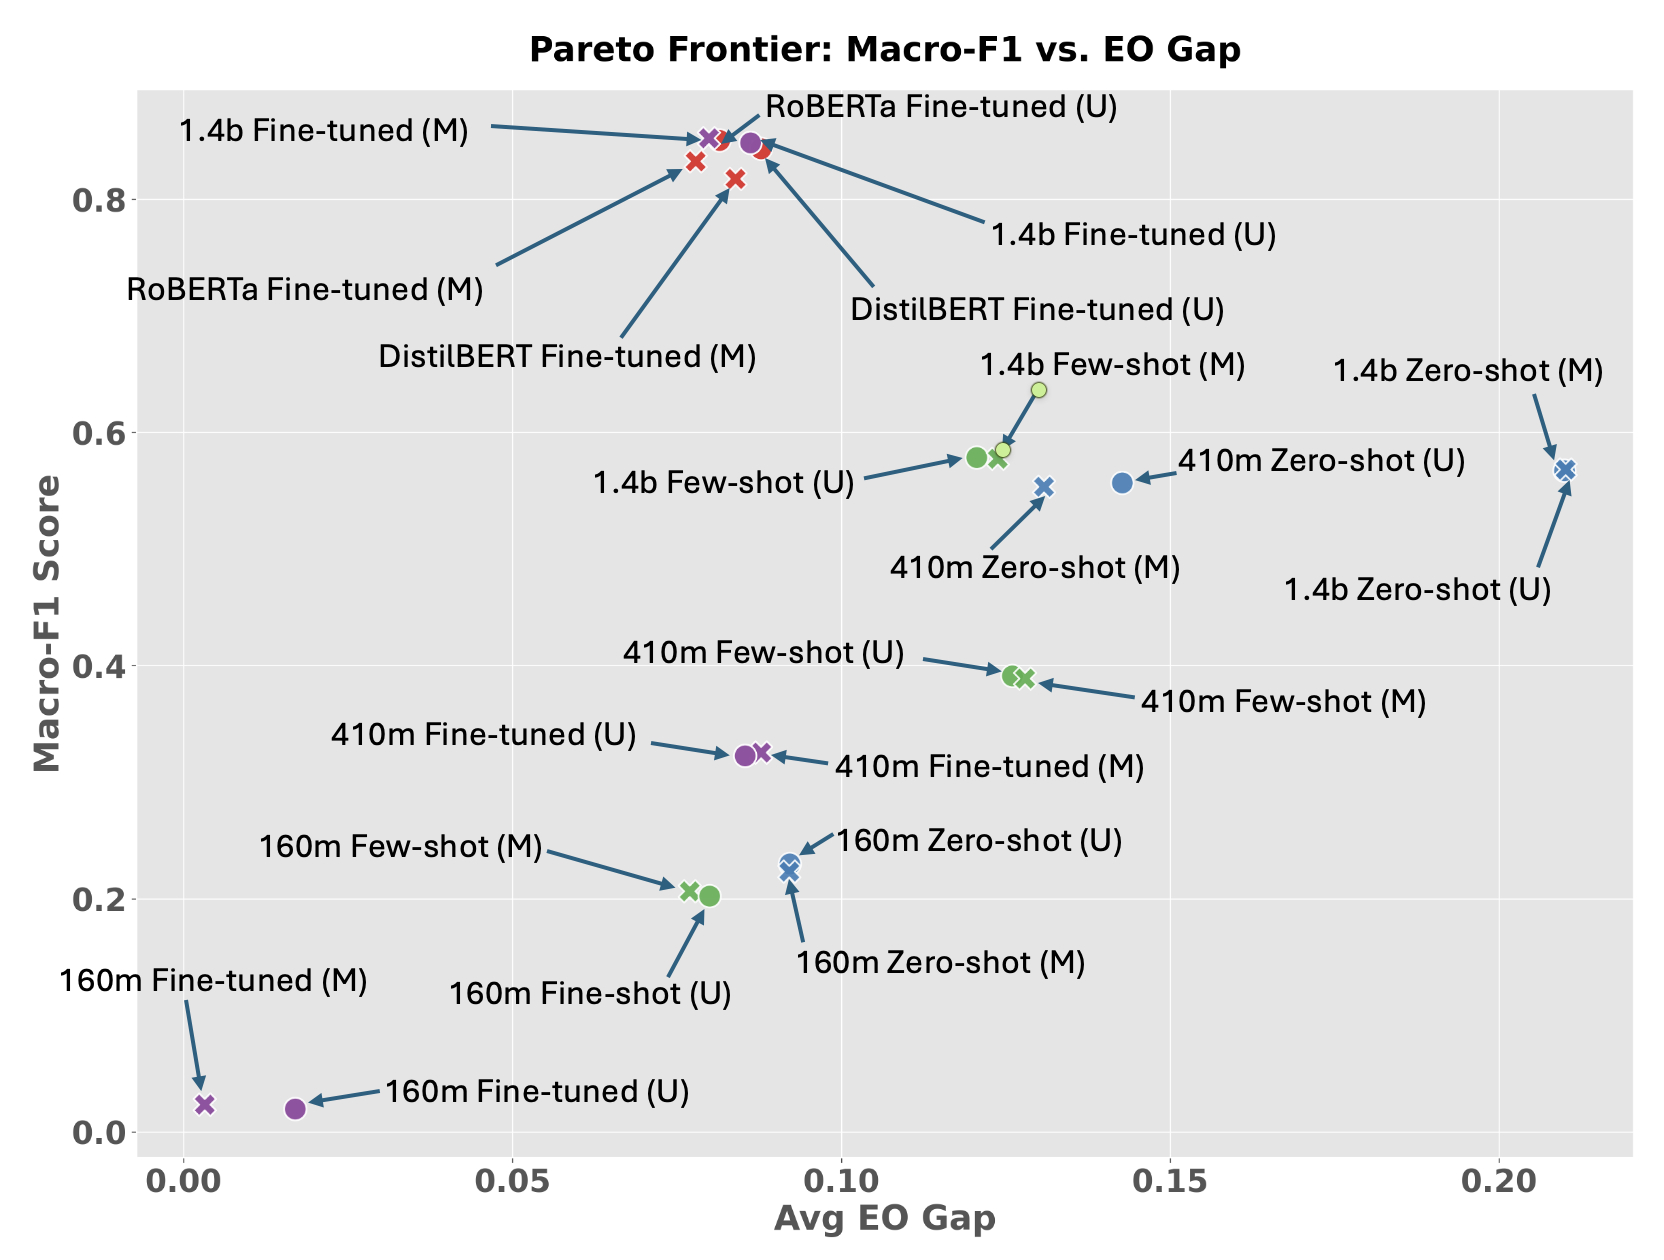
\includegraphics[width=\linewidth]{pareto_frontier_labelled.png}
\caption{Pareto frontier of Macro-F1 vs. Equalized Odds gap. RoBERTa masked fine-tuned, closely followed by Pythia-1.4B masked fine-tuned, is the most Pareto-optimal model. The generative models which are masked and with largest capacity, as well as the baseline encoders, strongly dominate lower-capacity, zero-shot and few-shot alternatives.}
\label{fig:pareto}
\end{figure}

\begin{figure}[h!]
\centering
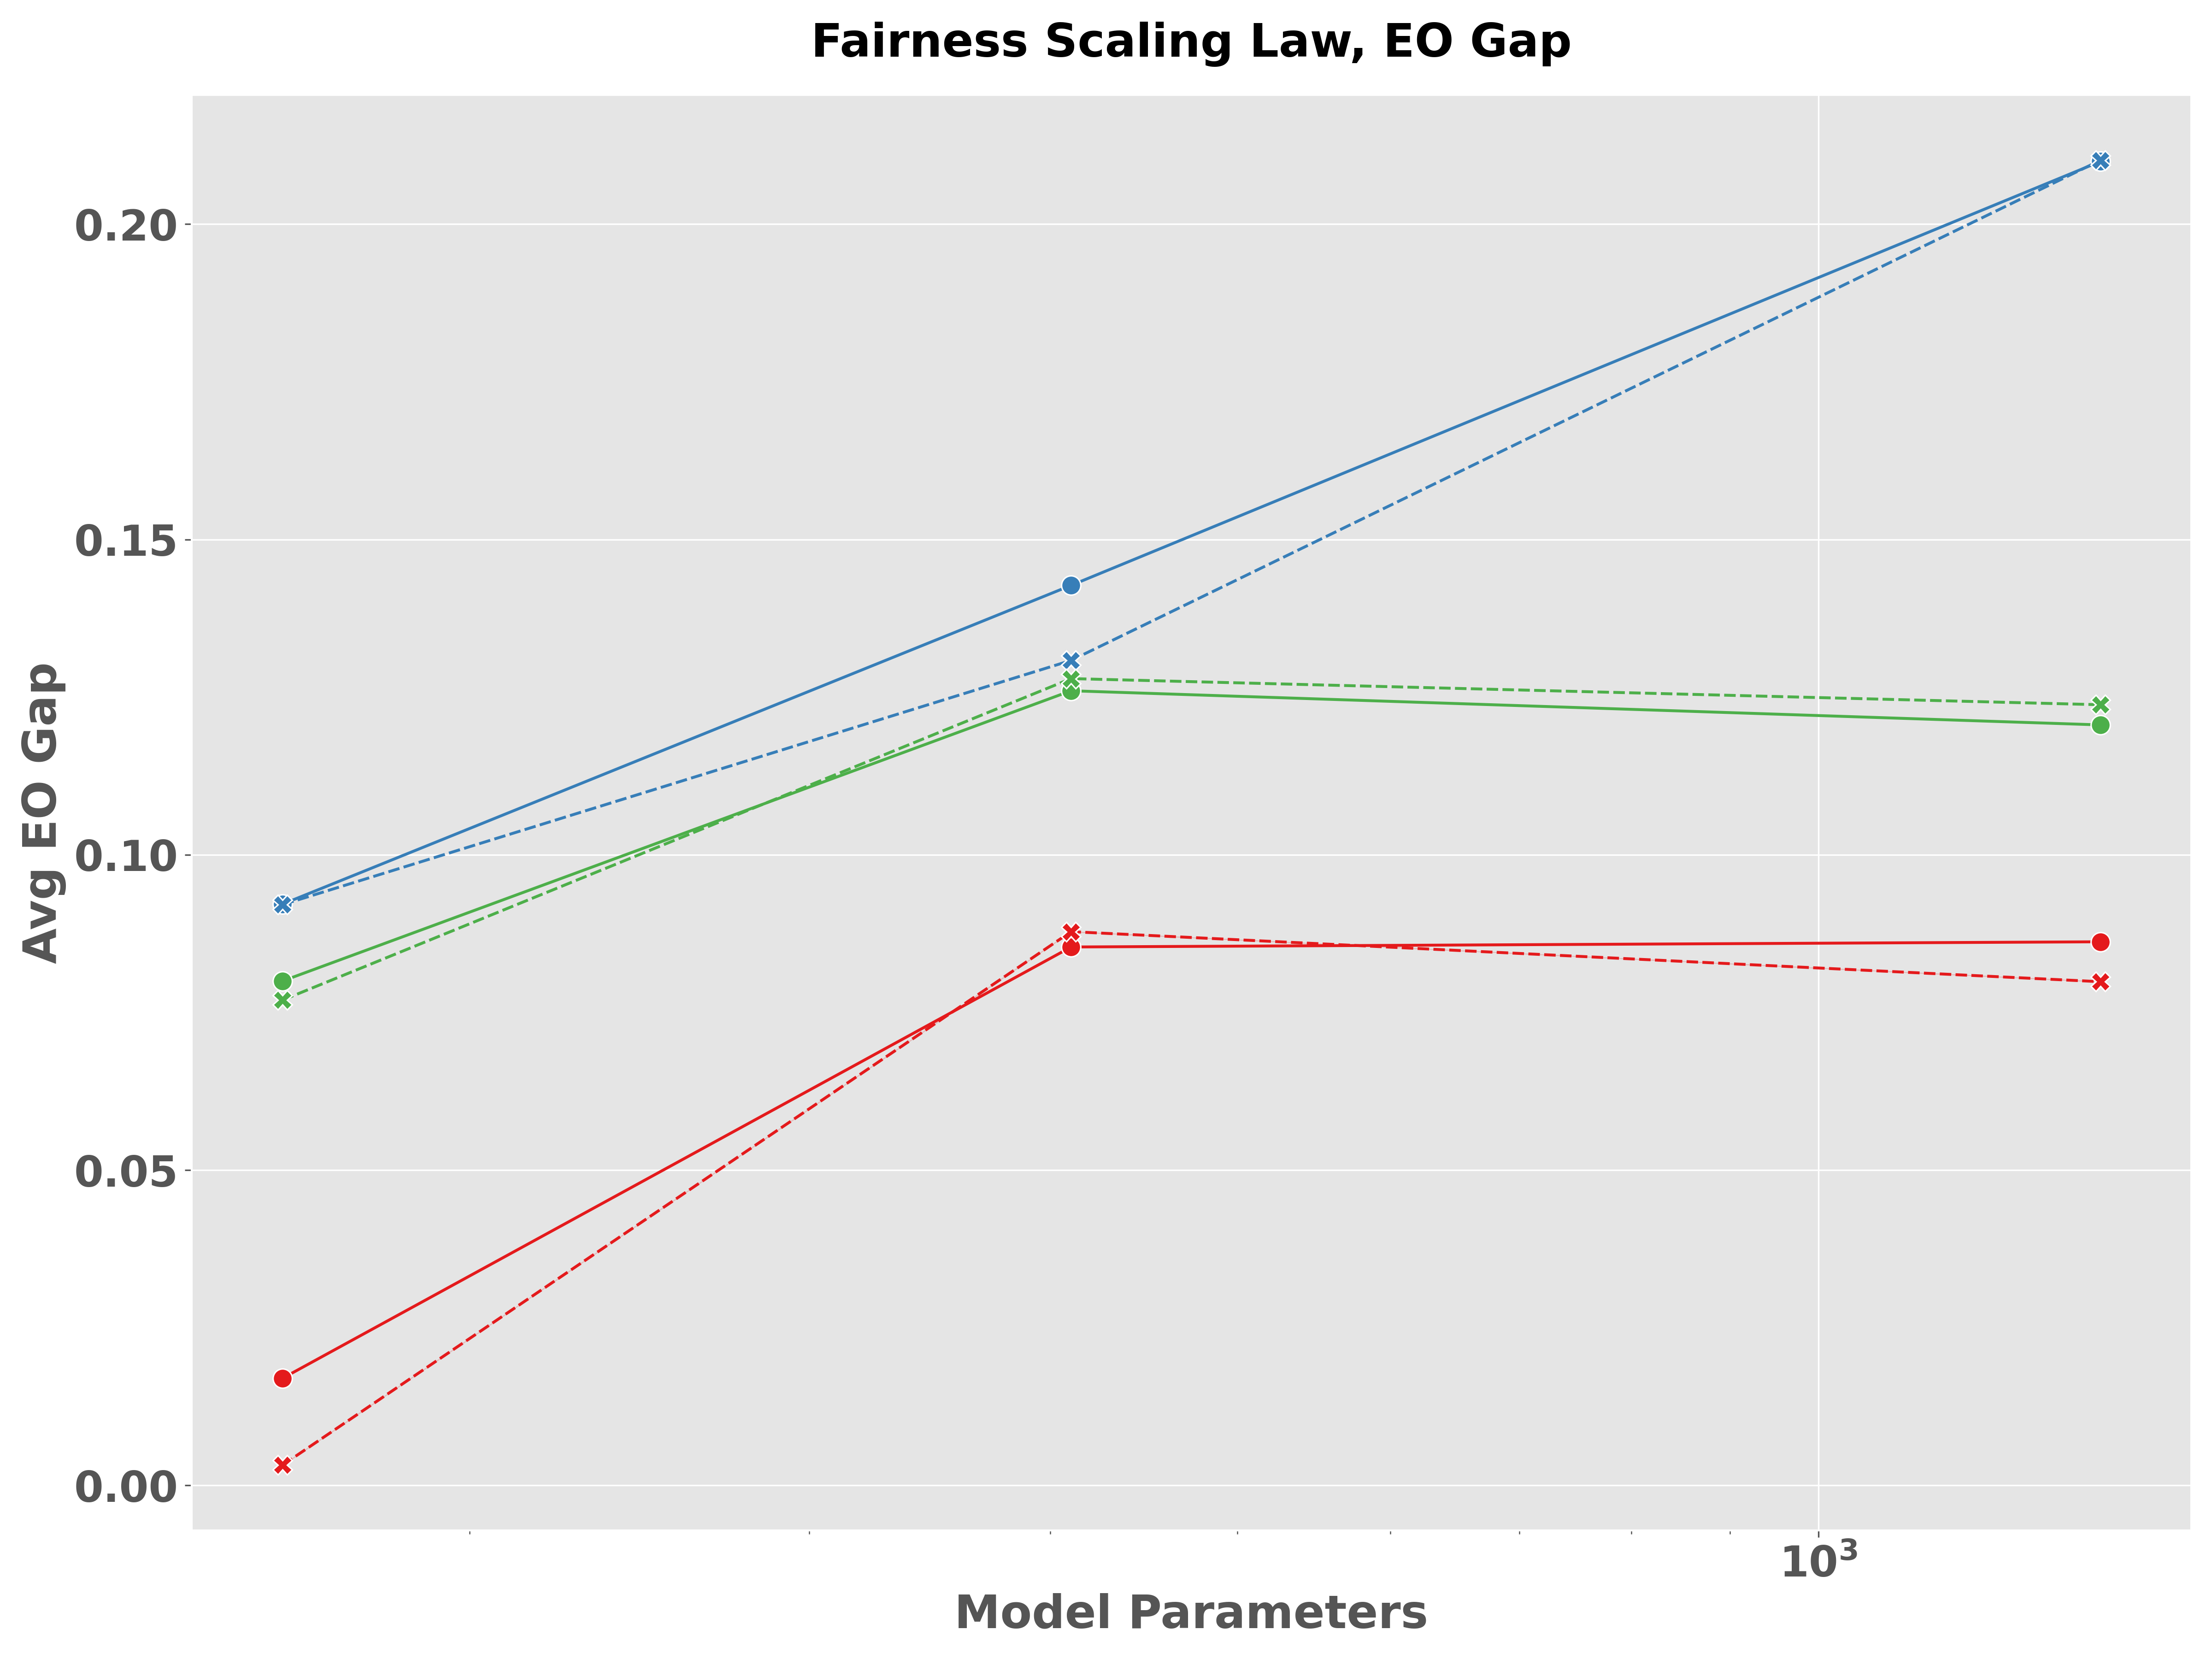
\includegraphics[width=\linewidth]{scaling_fairness.png}
\caption{Scaling behavior of Equalized Odds gap across model sizes, 1.4B (red), 410m (green), and 160m (blue). The solid line corresponds to unmasked, and dashed to masked). Zero-shot bias increases with scale, while fine-tuning mitigates this effect.}
\label{fig:scaling_fairness}
\end{figure}

\textbf{Fine-tuning substantially improves fairness.}
Fine-tuned models achieve markedly lower EO gaps than zero-shot
counterparts.

\textbf{Zero-shot bias increases with scale.}
EO gap increases from $\sim$0.09 (Pythia-160M) to $\sim$0.21
(Pythia-1.4B) in the zero-shot regime---larger models amplify
stereotypical associations without task-specific supervision.

\textbf{Masking provides modest but inconsistent improvement.}
For Pythia-1.4B fine-tuned, masking reduces EO gap from 0.086 to
0.080. The effect is non-uniform: masking reduces bias for
\emph{nurse}, \emph{surgeon}, and \emph{model}, but increases it for
\emph{teacher}, \emph{poet}, and \emph{painter} (backfire effect).

\textbf{TPR gap dominates FPR gap} across all models, as the EO column is equal to the TPR column. This indicates that the primary fairness issue lies in differential true positive rates across gender groups.
To understand why these disparities persist even under masking,
we turn to token-level attribution analysis.

\subsection{Proxy Bias Analysis}

We analyse which tokens drive occupation predictions and how their
importance shifts under gender masking. We first assess attribution
stability under masking, then examine which token types carry the
gender signal, and finally validate causal load-bearing via
faithfulness testing.

\begin{table}[h]
\centering\small
\begin{tabular}{lcc}
\toprule
\textbf{Profession} & \textbf{DistilBERT} & \textbf{RoBERTa} \\
\midrule
comedian          & 0.54 & 0.33 \\
dentist           & 0.54 & 0.33 \\
dietitian         & 0.67 & 0.54 \\
nurse             & 0.43 & 0.54 \\
psychologist      & 0.82 & 0.82 \\
software engineer & 0.67 & 0.43 \\
attorney          & 0.67 & 0.82 \\
journalist        & 0.67 & 0.67 \\
physician         & 0.67 & 0.54 \\
professor         & 0.82 & 1.00 \\
\bottomrule
\end{tabular}
\caption{Shared token ratio (masked vs.\ unmasked). Higher = more stable.}
\end{table}

Under RoBERTa, \emph{comedian} and \emph{dentist} are the most
unstable professions (ratio 0.33), while under DistilBERT both
are moderately stable (0.54)---the same reversal observed for
\emph{nurse} (DistilBERT 0.43, RoBERTa 0.54). \emph{Professor}
reaches maximum stability under RoBERTa (1.00), meaning its top-10
tokens are identical across masked and unmasked conditions. These
cross-profession reversals reinforce the conclusion that proxy
stability depends on the specific model, not only training data.

When gender tokens are removed, attribution is redistributed across
tokens rather than concentrated on the same dominant token, consistent
with the completeness property of Integrated Gradients.
The profession label token (e.g.\ \emph{nurse} for the nurse class)
frequently appears among the top-$K$ attributed tokens, reflecting
label leakage where the profession name occurs directly in the
biography. This is expected; the methodologically informative signal
lies in how attribution shifts between unmasked and masked conditions.
For DistilBERT on \emph{nurse}, the label token \emph{nurse}
remains prominent under both conditions (129.89 unmasked,
152.73 masked), consistent with label leakage noted above.
The informative shift occurs in secondary tokens: \emph{practitioner}
(26.51) and \emph{graduated} (19.11) drop out, while \emph{hospital}
(+8.96) and \emph{especially} (+15.52) gain importance.
For RoBERTa on \emph{physician}, masking shifts weight toward
higher-level clinical context: \emph{medicine} rises from 166.64
to 292.25 and \emph{patients} (52.72) emerges as a new signal,
while \emph{affiliated} (68.78 unmasked) drops from the top-5.

\begin{table}[h]
\centering\small
\setlength{\tabcolsep}{4pt}
\begin{tabular}{llcc}
\toprule
\textbf{Model} & \textbf{Token} & \textbf{Type} & \textbf{W.Score} \\
\midrule
DistilBERT & \emph{actor}  & gender & 1.15 \\
DistilBERT & \emph{sister} & gender & 1.13 \\
DistilBERT & \emph{mrs}    & gender & 1.05 \\
\midrule
RoBERTa & \emph{mrs}    & gender & 2.11 \\
RoBERTa & \emph{wife}   & gender & 0.78 \\
\midrule
RoBERTa & \emph{nursing}  & profession & 70.44 \\
RoBERTa & \emph{medicine} & profession & 166.64 \\
RoBERTa & \emph{research} & profession & 333.32 \\
\bottomrule
\end{tabular}
\caption{Attribution weight of gender tokens vs.\ profession tokens.
Gender tokens appear in both models but with substantially smaller
weights than dominant profession tokens.}
\end{table}

Under both models, a small number of explicit gender tokens appear
in the aggregated top-$K$ features, but with substantially smaller
weights than dominant profession tokens: DistilBERT's highest gender
token (\emph{actor}: 1.15) is over 100 times smaller than top
profession tokens (70--333), and RoBERTa's \emph{mrs} (2.11)
is similarly dwarfed. Bias likely operates primarily through
indirect contextual signals rather than explicit gender indicators.

Gender-conditioned analysis reveals partial asymmetry.
Under DistilBERT, nurse$|$F and nurse$|$M both retain 5 shared
tokens (ratio 0.33 each), showing no directional asymmetry.
Under RoBERTa, nurse$|$F retains 7 shared tokens (ratio 0.54)
versus nurse$|$M retaining 6 (ratio 0.43), a modest asymmetry
suggesting the learned feature space for \emph{nurse} is
somewhat more anchored in female-typical contextual patterns.
This attribution-level asymmetry aligns with the fairness results in
Section~\ref{sec:fairness}, where \emph{nurse} shows one of the
largest EO gap reductions under masking---suggesting that professions
with unstable proxy representations are precisely those where masking
provides the most benefit.

\subsubsection*{Faithfulness Validation}

While Integrated Gradients provides correlational insights into
feature importance, the top-$K$ erasure test constitutes an
intervention-based validation: erasing attributed tokens and
measuring the resulting confidence drop directly tests whether
those tokens are causally load-bearing for the prediction.
Table~\ref{tab:faithfulness} reports mean faithfulness scores by
profession across both models and masking conditions. Across all
3,000 examples, 89.6\% (DistilBERT) and 82.3\% (RoBERTa) of
predictions show positive faithfulness, confirming the attributed
tokens are genuinely load-bearing.

\begin{table}[h]
\centering\small
\setlength{\tabcolsep}{4pt}
\begin{tabular}{lcccc}
\toprule
\textbf{Profession} & \multicolumn{2}{c}{\textbf{DistilBERT}} & \multicolumn{2}{c}{\textbf{RoBERTa}} \\
& \textbf{U} & \textbf{M} & \textbf{U} & \textbf{M} \\
\midrule
Dietitian         & 0.619 & 0.743 & 0.548 & 0.372 \\
Nurse             & 0.395 & 0.518 & 0.203 & 0.197 \\
Psychologist      & 0.356 & 0.378 & 0.232 & 0.252 \\
Painter           & 0.473 & 0.418 & 0.339 & 0.342 \\
Physician         & 0.233 & 0.191 & 0.235 & 0.200 \\
Attorney          & 0.162 & 0.221 & 0.175 & 0.158 \\
Professor         & 0.160 & 0.214 & 0.162 & 0.182 \\
Software Engineer & 0.171 & 0.204 & 0.193 & 0.199 \\
\midrule
\textit{Overall}  & 0.330 & 0.364 & 0.243 & 0.249 \\
\bottomrule
\end{tabular}
\caption{Mean faithfulness (probability drop after erasing top-5
attributed tokens). U=unmasked; M=masked. Higher = more causally
load-bearing tokens. The \textit{Overall} row is the
macro-average across all 20 professions (equal weight per
profession, not per example).}
\label{tab:faithfulness}
\end{table}

Faithfulness scores align with the proxy stability analysis:
professions with lower shared ratios tend toward higher faithfulness
(\emph{dietitian}: 0.619, \emph{nurse}: 0.395), while stable
professions show lower faithfulness (\emph{professor}: 0.160,
\emph{attorney}: 0.162). This corroborates that attribution
instability identifies professions whose predictions depend on
concentrated, causally decisive feature sets. Notably, the
\emph{model} profession under RoBERTa unmasked achieves the lowest
faithfulness of all 20 professions (0.100), suggesting its
predictions are distributed across many weakly-attributing tokens
rather than a small decisive set.

Gender-conditioned faithfulness reveals a striking asymmetry for
\emph{nurse} under DistilBERT: nurse$|$M faithfulness = 0.756 versus
nurse$|$F = 0.354. Male nurse predictions are almost entirely driven
by the small set of attributed tokens --- erasing them nearly halves
the model's confidence. This corroborates the earlier finding that
male nurse representations lack stable content anchors.
Under RoBERTa the asymmetry is also present but larger in magnitude:
nurse$|$M = 0.534 versus nurse$|$F = 0.163. Full gender-conditioned faithfulness results for all professions are reported in Appendix~D.

Masking increases overall faithfulness for both models (DistilBERT:
+0.034; RoBERTa: +0.006), indicating that after gender signals are
removed, the remaining attributed tokens become more causally decisive
--- the model concentrates its predictions on a smaller, more critical
feature set.

% ── 7. CONCLUSION ───────────────────────────────────────────────
\section{Conclusion}

Fine-tuned models substantially outperform zero/few-shot baselines in both performance and fairness; scaling without supervision amplifies bias; masking provides modest and non-uniform improvement; and bias is encoded primarily through indirect contextual tokens whose 
importance is model-dependent and whose causal load is supported by 
erasure faithfulness testing.
Notably, zero-shot EO gap grows from $\sim$0.09 at 160M to $\sim$0.21
at 1.4B parameters---suggesting that model capacity alone is not a
substitute for task-specific fine-tuning or explicit debiasing interventions.
Gender-conditioned analysis further reveals that male nurse
predictions are disproportionately dependent on a critically
small feature set, with faithfulness nearly double that of
female nurse predictions (0.756 vs.\ 0.354 under DistilBERT).

\paragraph{Limitations.}
The dataset provides binary gender labels inferred from pronoun 
usage by the original authors \citep{de-arteaga-etal-2019-bias}, 
which do not capture the full spectrum of gender identity and 
limit fairness evaluation to a male/female binary. Attribution is restricted to encoder
models. Per-profession evaluation uses proportional
stratification from the 3,000-sample canonical subset, resulting in
small sample sizes for low-frequency professions (e.g.\ comedian
$n\!=\!27$, dietitian $n\!=\!30$); per-profession fairness estimates
for these occupations should be interpreted with caution.

\paragraph{Future work.}
Remaining directions include a formal cross-gender proxy bias score and extending attribution to generative models.

% ── APPENDICES ──────────────────────────────────────────────────
\appendix


\section{Per-Occupation Proxy Word Tables}
\noindent Top-5 attributed tokens (weighted score = count\_topk $\times$ mean attribution)
per profession for DistilBERT and RoBERTa under unmasked (U) and masked (M) conditions.
Aggregated over 3,000 test examples; stopwords and tokens shorter than 3 characters excluded.
\textit{Note: some RoBERTa entries (e.g.\ \emph{olog}, \emph{ession}, \emph{ition}) reflect
BPE subword fragments and should be interpreted as components of larger lexical units.}


\vspace{4pt}\noindent\textbf{Accountant}
\begin{center}\scriptsize
\begin{tabular}{lrllr}
\toprule
\multicolumn{2}{c}{\textbf{DistilBERT (U/M)}} & & \multicolumn{2}{c}{\textbf{RoBERTa (U/M)}} \\
\textbf{Token} & \textbf{W.Score} & & \textbf{Token} & \textbf{W.Score} \\
\midrule
\multicolumn{5}{l}{\textit{Unmasked}} \\
\emph{accounting} & 20.8 & & \emph{accounting} & 17.8 \\
\emph{financial} & 9.5 & & \emph{financial} & 9.2 \\
\emph{accounts} & 3.9 & & \emph{account} & 7.0 \\
\emph{finance} & 3.1 & & \emph{business} & 6.4 \\
\emph{tax} & 2.1 & & \emph{tax} & 5.6 \\
\multicolumn{5}{l}{\textit{Masked}} \\
\emph{accounting} & 21.4 & & \emph{accounting} & 18.3 \\
\emph{financial} & 10.6 & & \emph{financial} & 10.3 \\
\emph{accounts} & 4.0 & & \emph{account} & 9.0 \\
\emph{finance} & 4.0 & & \emph{business} & 8.2 \\
\emph{tax} & 2.2 & & \emph{finance} & 5.1 \\
\bottomrule
\end{tabular}
\end{center}

\vspace{4pt}\noindent\textbf{Architect}
\begin{center}\scriptsize
\begin{tabular}{lrllr}
\toprule
\multicolumn{2}{c}{\textbf{DistilBERT (U/M)}} & & \multicolumn{2}{c}{\textbf{RoBERTa (U/M)}} \\
\textbf{Token} & \textbf{W.Score} & & \textbf{Token} & \textbf{W.Score} \\
\midrule
\multicolumn{5}{l}{\textit{Unmasked}} \\
\emph{architecture} & 29.4 & & \emph{architecture} & 43.5 \\
\emph{architectural} & 15.7 & & \emph{design} & 21.3 \\
\emph{design} & 13.0 & & \emph{architect} & 20.6 \\
\emph{architect} & 11.1 & & \emph{architectural} & 13.0 \\
\emph{architects} & 7.9 & & \emph{architects} & 9.0 \\
\multicolumn{5}{l}{\textit{Masked}} \\
\emph{architecture} & 27.8 & & \emph{architecture} & 38.7 \\
\emph{architectural} & 15.1 & & \emph{design} & 20.4 \\
\emph{design} & 13.6 & & \emph{architects} & 13.3 \\
\emph{architects} & 8.8 & & \emph{architectural} & 12.1 \\
\emph{construction} & 4.1 & & \emph{architect} & 11.9 \\
\bottomrule
\end{tabular}
\end{center}

\vspace{4pt}\noindent\textbf{Attorney}
\begin{center}\scriptsize
\begin{tabular}{lrllr}
\toprule
\multicolumn{2}{c}{\textbf{DistilBERT (U/M)}} & & \multicolumn{2}{c}{\textbf{RoBERTa (U/M)}} \\
\textbf{Token} & \textbf{W.Score} & & \textbf{Token} & \textbf{W.Score} \\
\midrule
\multicolumn{5}{l}{\textit{Unmasked}} \\
\emph{law} & 53.3 & & \emph{law} & 183.4 \\
\emph{attorney} & 37.1 & & \emph{attorney} & 54.9 \\
\emph{legal} & 26.9 & & \emph{litigation} & 51.5 \\
\emph{litigation} & 25.0 & & \emph{legal} & 46.3 \\
\emph{clients} & 19.7 & & \emph{practice} & 42.9 \\
\multicolumn{5}{l}{\textit{Masked}} \\
\emph{law} & 56.9 & & \emph{law} & 168.8 \\
\emph{legal} & 28.6 & & \emph{legal} & 56.7 \\
\emph{litigation} & 25.3 & & \emph{litigation} & 53.8 \\
\emph{clients} & 19.7 & & \emph{practice} & 31.4 \\
\emph{counsel} & 18.8 & & \emph{court} & 21.9 \\
\bottomrule
\end{tabular}
\end{center}

\vspace{4pt}\noindent\textbf{Comedian}
\begin{center}\scriptsize
\begin{tabular}{lrllr}
\toprule
\multicolumn{2}{c}{\textbf{DistilBERT (U/M)}} & & \multicolumn{2}{c}{\textbf{RoBERTa (U/M)}} \\
\textbf{Token} & \textbf{W.Score} & & \textbf{Token} & \textbf{W.Score} \\
\midrule
\multicolumn{5}{l}{\textit{Unmasked}} \\
\emph{comedy} & 16.4 & & \emph{comedy} & 16.7 \\
\emph{stand} & 4.3 & & \emph{stand} & 6.5 \\
\emph{comedians} & 2.9 & & \emph{comedians} & 5.8 \\
\emph{performed} & 2.0 & & \emph{performed} & 2.1 \\
-- & -- & & \emph{show} & 1.5 \\
\multicolumn{5}{l}{\textit{Masked}} \\
\emph{comedy} & 16.7 & & \emph{comedy} & 19.0 \\
\emph{stand} & 3.8 & & \emph{comedians} & 6.1 \\
\emph{comedians} & 3.1 & & \emph{stand} & 4.9 \\
\emph{funny} & 2.4 & & \emph{show} & 1.4 \\
\emph{performed} & 1.8 & & -- & -- \\
\bottomrule
\end{tabular}
\end{center}

\vspace{4pt}\noindent\textbf{Composer}
\begin{center}\scriptsize
\begin{tabular}{lrllr}
\toprule
\multicolumn{2}{c}{\textbf{DistilBERT (U/M)}} & & \multicolumn{2}{c}{\textbf{RoBERTa (U/M)}} \\
\textbf{Token} & \textbf{W.Score} & & \textbf{Token} & \textbf{W.Score} \\
\midrule
\multicolumn{5}{l}{\textit{Unmasked}} \\
\emph{music} & 23.9 & & \emph{music} & 28.6 \\
\emph{composition} & 6.4 & & \emph{composition} & 7.2 \\
\emph{composer} & 6.3 & & \emph{scores} & 7.1 \\
\emph{musical} & 5.0 & & \emph{musical} & 6.8 \\
\emph{composing} & 4.2 & & \emph{compositions} & 6.7 \\
\multicolumn{5}{l}{\textit{Masked}} \\
\emph{music} & 23.9 & & \emph{music} & 27.3 \\
\emph{composition} & 7.2 & & \emph{composition} & 10.1 \\
\emph{compositions} & 5.3 & & \emph{scores} & 6.6 \\
\emph{musical} & 5.0 & & \emph{musical} & 6.0 \\
\emph{composing} & 3.9 & & \emph{composing} & 5.6 \\
\bottomrule
\end{tabular}
\end{center}

\vspace{4pt}\noindent\textbf{Dentist}
\begin{center}\scriptsize
\begin{tabular}{lrllr}
\toprule
\multicolumn{2}{c}{\textbf{DistilBERT (U/M)}} & & \multicolumn{2}{c}{\textbf{RoBERTa (U/M)}} \\
\textbf{Token} & \textbf{W.Score} & & \textbf{Token} & \textbf{W.Score} \\
\midrule
\multicolumn{5}{l}{\textit{Unmasked}} \\
\emph{dental} & 105.5 & & \emph{ental} & 90.5 \\
\emph{dentistry} & 48.8 & & \emph{dent} & 45.7 \\
\emph{dentist} & 28.3 & & \emph{dental} & 33.4 \\
\emph{bds} & 23.2 & & \emph{clinic} & 22.7 \\
\emph{clinic} & 9.6 & & \emph{patients} & 21.1 \\
\multicolumn{5}{l}{\textit{Masked}} \\
\emph{dental} & 125.2 & & \emph{ental} & 94.5 \\
\emph{dentistry} & 49.9 & & \emph{dental} & 39.8 \\
\emph{bds} & 18.7 & & \emph{dent} & 33.0 \\
\emph{clinic} & 11.4 & & \emph{clinic} & 23.0 \\
\emph{patients} & 9.2 & & \emph{patients} & 19.4 \\
\bottomrule
\end{tabular}
\end{center}

\vspace{4pt}\noindent\textbf{Dietitian}
\begin{center}\scriptsize
\begin{tabular}{lrllr}
\toprule
\multicolumn{2}{c}{\textbf{DistilBERT (U/M)}} & & \multicolumn{2}{c}{\textbf{RoBERTa (U/M)}} \\
\textbf{Token} & \textbf{W.Score} & & \textbf{Token} & \textbf{W.Score} \\
\midrule
\multicolumn{5}{l}{\textit{Unmasked}} \\
\emph{nutrition} & 37.4 & & \emph{nutrition} & 24.7 \\
\emph{dietitian} & 35.1 & & \emph{diet} & 4.9 \\
\emph{registered} & 6.4 & & \emph{ession} & 4.3 \\
\emph{nutritional} & 3.9 & & \emph{nutritional} & 3.8 \\
\emph{diet} & 3.1 & & \emph{health} & 2.2 \\
\multicolumn{5}{l}{\textit{Masked}} \\
\emph{nutrition} & 57.3 & & \emph{nutrition} & 20.8 \\
\emph{having} & 4.4 & & \emph{ession} & 7.1 \\
\emph{experiences} & 3.8 & & \emph{diet} & 4.5 \\
\emph{nutritional} & 3.5 & & \emph{nutritional} & 4.0 \\
\emph{diet} & 3.4 & & \emph{specializes} & 2.7 \\
\bottomrule
\end{tabular}
\end{center}

\vspace{4pt}\noindent\textbf{Filmmaker}
\begin{center}\scriptsize
\begin{tabular}{lrllr}
\toprule
\multicolumn{2}{c}{\textbf{DistilBERT (U/M)}} & & \multicolumn{2}{c}{\textbf{RoBERTa (U/M)}} \\
\textbf{Token} & \textbf{W.Score} & & \textbf{Token} & \textbf{W.Score} \\
\midrule
\multicolumn{5}{l}{\textit{Unmasked}} \\
\emph{film} & 20.7 & & \emph{film} & 26.4 \\
\emph{films} & 12.2 & & \emph{films} & 24.9 \\
\emph{documentary} & 8.5 & & \emph{feature} & 7.8 \\
\emph{filmmaking} & 7.8 & & \emph{filmmaker} & 7.2 \\
\emph{directed} & 4.5 & & \emph{filmmaking} & 6.9 \\
\multicolumn{5}{l}{\textit{Masked}} \\
\emph{film} & 21.4 & & \emph{film} & 27.4 \\
\emph{films} & 11.7 & & \emph{films} & 20.9 \\
\emph{filmmaking} & 7.2 & & \emph{filmmaking} & 6.6 \\
\emph{documentary} & 5.7 & & \emph{documentary} & 5.8 \\
\emph{directed} & 5.2 & & \emph{festivals} & 5.4 \\
\bottomrule
\end{tabular}
\end{center}

\vspace{4pt}\noindent\textbf{Journalist}
\begin{center}\scriptsize
\begin{tabular}{lrllr}
\toprule
\multicolumn{2}{c}{\textbf{DistilBERT (U/M)}} & & \multicolumn{2}{c}{\textbf{RoBERTa (U/M)}} \\
\textbf{Token} & \textbf{W.Score} & & \textbf{Token} & \textbf{W.Score} \\
\midrule
\multicolumn{5}{l}{\textit{Unmasked}} \\
\emph{journalism} & 34.5 & & \emph{journalism} & 32.0 \\
\emph{journalist} & 17.9 & & \emph{news} & 19.6 \\
\emph{news} & 12.9 & & \emph{journalist} & 15.7 \\
\emph{editor} & 11.4 & & \emph{editor} & 13.7 \\
\emph{journalists} & 8.4 & & \emph{reporting} & 8.9 \\
\multicolumn{5}{l}{\textit{Masked}} \\
\emph{journalism} & 35.3 & & \emph{journalism} & 36.1 \\
\emph{news} & 14.4 & & \emph{news} & 23.4 \\
\emph{editor} & 12.5 & & \emph{editor} & 10.8 \\
\emph{journalists} & 7.8 & & \emph{times} & 10.4 \\
\emph{reporting} & 7.4 & & \emph{reporting} & 10.0 \\
\bottomrule
\end{tabular}
\end{center}

\vspace{4pt}\noindent\textbf{Model}
{\scriptsize\textit{Note: \emph{freeones} is a website name from the training corpus, not a profession descriptor --- an example of dataset artefacts appearing in proxy tables.}}
\begin{center}\scriptsize
\begin{tabular}{lrllr}
\toprule
\multicolumn{2}{c}{\textbf{DistilBERT (U/M)}} & & \multicolumn{2}{c}{\textbf{RoBERTa (U/M)}} \\
\textbf{Token} & \textbf{W.Score} & & \textbf{Token} & \textbf{W.Score} \\
\midrule
\multicolumn{5}{l}{\textit{Unmasked}} \\
\emph{model} & 16.4 & & \emph{model} & 28.1 \\
\emph{freeones} & 15.2 & & \emph{born} & 20.8 \\
\emph{modeling} & 14.0 & & \emph{modeling} & 13.9 \\
\emph{born} & 7.1 & & \emph{currently} & 6.7 \\
\emph{gallery} & 5.3 & & \emph{fashion} & 6.5 \\
\multicolumn{5}{l}{\textit{Masked}} \\
\emph{freeones} & 22.7 & & \emph{modeling} & 17.7 \\
\emph{modeling} & 15.2 & & \emph{gallery} & 8.5 \\
\emph{born} & 8.0 & & \emph{modelling} & 8.4 \\
\emph{gallery} & 5.8 & & \emph{currently} & 8.4 \\
\emph{modelling} & 4.6 & & \emph{ranked} & 6.3 \\
\bottomrule
\end{tabular}
\end{center}

\vspace{4pt}\noindent\textbf{Nurse}
\begin{center}\scriptsize
\begin{tabular}{lrllr}
\toprule
\multicolumn{2}{c}{\textbf{DistilBERT (U/M)}} & & \multicolumn{2}{c}{\textbf{RoBERTa (U/M)}} \\
\textbf{Token} & \textbf{W.Score} & & \textbf{Token} & \textbf{W.Score} \\
\midrule
\multicolumn{5}{l}{\textit{Unmasked}} \\
\emph{nurse} & 127.3 & & \emph{nursing} & 91.5 \\
\emph{nursing} & 54.6 & & \emph{nurse} & 76.2 \\
\emph{practitioner} & 25.1 & & \emph{specialists} & 24.2 \\
\emph{graduated} & 20.5 & & \emph{graduated} & 23.2 \\
\emph{experiences} & 14.5 & & \emph{medical} & 21.8 \\
\multicolumn{5}{l}{\textit{Masked}} \\
\emph{nursing} & 66.6 & & \emph{nursing} & 107.5 \\
\emph{graduated} & 23.0 & & \emph{medical} & 20.3 \\
\emph{nurse} & 8.9 & & \emph{doctors} & 17.4 \\
\emph{nurses} & 7.6 & & \emph{ition} & 16.9 \\
\emph{medicine} & 7.2 & & \emph{health} & 15.6 \\
\bottomrule
\end{tabular}
\end{center}

\vspace{4pt}\noindent\textbf{Painter}
\begin{center}\scriptsize
\begin{tabular}{lrllr}
\toprule
\multicolumn{2}{c}{\textbf{DistilBERT (U/M)}} & & \multicolumn{2}{c}{\textbf{RoBERTa (U/M)}} \\
\textbf{Token} & \textbf{W.Score} & & \textbf{Token} & \textbf{W.Score} \\
\midrule
\multicolumn{5}{l}{\textit{Unmasked}} \\
\emph{paintings} & 25.4 & & \emph{painting} & 41.5 \\
\emph{painting} & 21.1 & & \emph{paintings} & 38.8 \\
\emph{gallery} & 8.1 & & \emph{art} & 9.6 \\
\emph{art} & 7.8 & & \emph{paint} & 8.6 \\
\emph{paint} & 4.1 & & \emph{gallery} & 7.2 \\
\multicolumn{5}{l}{\textit{Masked}} \\
\emph{paintings} & 23.8 & & \emph{painting} & 36.7 \\
\emph{painting} & 22.1 & & \emph{paintings} & 35.4 \\
\emph{art} & 8.7 & & \emph{art} & 11.9 \\
\emph{gallery} & 7.1 & & \emph{paint} & 8.6 \\
\emph{paint} & 4.1 & & \emph{gallery} & 6.2 \\
\bottomrule
\end{tabular}
\end{center}

\vspace{4pt}\noindent\textbf{Photographer}
\begin{center}\scriptsize
\begin{tabular}{lrllr}
\toprule
\multicolumn{2}{c}{\textbf{DistilBERT (U/M)}} & & \multicolumn{2}{c}{\textbf{RoBERTa (U/M)}} \\
\textbf{Token} & \textbf{W.Score} & & \textbf{Token} & \textbf{W.Score} \\
\midrule
\multicolumn{5}{l}{\textit{Unmasked}} \\
\emph{photography} & 146.1 & & \emph{photography} & 164.7 \\
\emph{photographs} & 25.5 & & \emph{photographs} & 32.9 \\
\emph{photographer} & 22.9 & & \emph{photographer} & 26.8 \\
\emph{photographic} & 15.9 & & \emph{images} & 18.9 \\
\emph{photo} & 14.3 & & \emph{photographic} & 17.8 \\
\multicolumn{5}{l}{\textit{Masked}} \\
\emph{photography} & 153.9 & & \emph{photography} & 176.8 \\
\emph{photographs} & 24.4 & & \emph{photographs} & 30.8 \\
\emph{photo} & 17.8 & & \emph{images} & 17.1 \\
\emph{photographic} & 17.0 & & \emph{photo} & 17.1 \\
\emph{images} & 10.1 & & \emph{photographic} & 16.5 \\
\bottomrule
\end{tabular}
\end{center}

\vspace{4pt}\noindent\textbf{Physician}
\begin{center}\scriptsize
\begin{tabular}{lrllr}
\toprule
\multicolumn{2}{c}{\textbf{DistilBERT (U/M)}} & & \multicolumn{2}{c}{\textbf{RoBERTa (U/M)}} \\
\textbf{Token} & \textbf{W.Score} & & \textbf{Token} & \textbf{W.Score} \\
\midrule
\multicolumn{5}{l}{\textit{Unmasked}} \\
\emph{medicine} & 262.6 & & \emph{medicine} & 203.5 \\
\emph{practices} & 77.5 & & \emph{practices} & 172.6 \\
\emph{medical} & 64.1 & & \emph{medical} & 110.4 \\
\emph{physician} & 36.1 & & \emph{specializes} & 45.8 \\
\emph{graduate} & 16.7 & & \emph{affiliated} & 41.7 \\
\multicolumn{5}{l}{\textit{Masked}} \\
\emph{medicine} & 238.6 & & \emph{practices} & 148.7 \\
\emph{practices} & 101.1 & & \emph{medicine} & 121.6 \\
\emph{medical} & 63.0 & & \emph{medical} & 106.7 \\
\emph{specializes} & 29.1 & & \emph{affiliated} & 79.5 \\
\emph{graduate} & 17.0 & & \emph{specializes} & 46.4 \\
\bottomrule
\end{tabular}
\end{center}

\vspace{4pt}\noindent\textbf{Poet}
\begin{center}\scriptsize
\begin{tabular}{lrllr}
\toprule
\multicolumn{2}{c}{\textbf{DistilBERT (U/M)}} & & \multicolumn{2}{c}{\textbf{RoBERTa (U/M)}} \\
\textbf{Token} & \textbf{W.Score} & & \textbf{Token} & \textbf{W.Score} \\
\midrule
\multicolumn{5}{l}{\textit{Unmasked}} \\
\emph{poetry} & 34.5 & & \emph{poetry} & 40.4 \\
\emph{poems} & 8.1 & & \emph{poems} & 19.7 \\
\emph{writing} & 4.4 & & \emph{writing} & 10.0 \\
\emph{english} & 3.0 & & \emph{poem} & 8.3 \\
\emph{poem} & 3.0 & & \emph{published} & 6.2 \\
\multicolumn{5}{l}{\textit{Masked}} \\
\emph{poetry} & 35.9 & & \emph{poetry} & 47.3 \\
\emph{poems} & 8.3 & & \emph{poems} & 18.8 \\
\emph{writing} & 4.7 & & \emph{writing} & 13.5 \\
\emph{poem} & 3.5 & & \emph{etry} & 6.3 \\
\emph{english} & 3.2 & & \emph{poem} & 6.1 \\
\bottomrule
\end{tabular}
\end{center}

\vspace{4pt}\noindent\textbf{Professor}
\begin{center}\scriptsize
\begin{tabular}{lrllr}
\toprule
\multicolumn{2}{c}{\textbf{DistilBERT (U/M)}} & & \multicolumn{2}{c}{\textbf{RoBERTa (U/M)}} \\
\textbf{Token} & \textbf{W.Score} & & \textbf{Token} & \textbf{W.Score} \\
\midrule
\multicolumn{5}{l}{\textit{Unmasked}} \\
\emph{research} & 322.9 & & \emph{research} & 364.0 \\
\emph{phd} & 92.0 & & \emph{phd} & 127.4 \\
\emph{interests} & 58.8 & & \emph{university} & 126.5 \\
\emph{university} & 58.6 & & \emph{interests} & 83.1 \\
\emph{focuses} & 48.0 & & \emph{teaching} & 67.5 \\
\multicolumn{5}{l}{\textit{Masked}} \\
\emph{research} & 220.1 & & \emph{research} & 302.4 \\
\emph{phd} & 69.9 & & \emph{university} & 135.8 \\
\emph{university} & 66.5 & & \emph{phd} & 100.4 \\
\emph{interests} & 58.0 & & \emph{interests} & 68.0 \\
\emph{focuses} & 50.2 & & \emph{faculty} & 63.5 \\
\bottomrule
\end{tabular}
\end{center}

\vspace{4pt}\noindent\textbf{Psychologist}
\begin{center}\scriptsize
\begin{tabular}{lrllr}
\toprule
\multicolumn{2}{c}{\textbf{DistilBERT (U/M)}} & & \multicolumn{2}{c}{\textbf{RoBERTa (U/M)}} \\
\textbf{Token} & \textbf{W.Score} & & \textbf{Token} & \textbf{W.Score} \\
\midrule
\multicolumn{5}{l}{\textit{Unmasked}} \\
\emph{psychologist} & 58.3 & & \emph{psychology} & 35.9 \\
\emph{psychology} & 42.0 & & \emph{olog} & 30.0 \\
\emph{psychological} & 9.1 & & \emph{clinical} & 13.2 \\
\emph{psychotherapy} & 9.1 & & \emph{psych} & 12.3 \\
\emph{experiences} & 8.0 & & \emph{psychological} & 10.5 \\
\multicolumn{5}{l}{\textit{Masked}} \\
\emph{psychology} & 42.1 & & \emph{psychology} & 36.8 \\
\emph{psychological} & 16.3 & & \emph{psychological} & 18.3 \\
\emph{psychotherapy} & 9.5 & & \emph{psych} & 11.7 \\
\emph{depression} & 9.2 & & \emph{clinical} & 11.1 \\
\emph{therapy} & 6.4 & & \emph{ical} & 10.8 \\
\bottomrule
\end{tabular}
\end{center}

\vspace{4pt}\noindent\textbf{Software Engineer}
\begin{center}\scriptsize
\begin{tabular}{lrllr}
\toprule
\multicolumn{2}{c}{\textbf{DistilBERT (U/M)}} & & \multicolumn{2}{c}{\textbf{RoBERTa (U/M)}} \\
\textbf{Token} & \textbf{W.Score} & & \textbf{Token} & \textbf{W.Score} \\
\midrule
\multicolumn{5}{l}{\textit{Unmasked}} \\
\emph{development} & 5.2 & & \emph{development} & 9.3 \\
\emph{engineering} & 4.6 & & \emph{engineering} & 9.2 \\
\emph{software} & 4.2 & & \emph{computer} & 7.0 \\
\emph{ibm} & 2.9 & & \emph{software} & 5.0 \\
\emph{developer} & 2.7 & & \emph{java} & 3.7 \\
\multicolumn{5}{l}{\textit{Masked}} \\
\emph{engineering} & 5.5 & & \emph{development} & 12.3 \\
\emph{development} & 4.8 & & \emph{engineering} & 7.8 \\
\emph{software} & 3.9 & & \emph{software} & 5.2 \\
\emph{ibm} & 2.9 & & \emph{computer} & 4.5 \\
\emph{code} & 2.4 & & \emph{building} & 3.2 \\
\bottomrule
\end{tabular}
\end{center}

\vspace{4pt}\noindent\textbf{Surgeon}
\begin{center}\scriptsize
\begin{tabular}{lrllr}
\toprule
\multicolumn{2}{c}{\textbf{DistilBERT (U/M)}} & & \multicolumn{2}{c}{\textbf{RoBERTa (U/M)}} \\
\textbf{Token} & \textbf{W.Score} & & \textbf{Token} & \textbf{W.Score} \\
\midrule
\multicolumn{5}{l}{\textit{Unmasked}} \\
\emph{surgery} & 43.7 & & \emph{surgery} & 83.7 \\
\emph{medical} & 13.2 & & \emph{medical} & 27.8 \\
\emph{medicine} & 11.7 & & \emph{surgeon} & 12.5 \\
\emph{practices} & 8.5 & & \emph{hospital} & 9.0 \\
\emph{surgeon} & 7.7 & & \emph{surgeries} & 8.9 \\
\multicolumn{5}{l}{\textit{Masked}} \\
\emph{surgery} & 42.6 & & \emph{surgery} & 80.4 \\
\emph{practices} & 10.5 & & \emph{medical} & 33.2 \\
\emph{medicine} & 8.9 & & \emph{practices} & 12.9 \\
\emph{medical} & 8.6 & & \emph{hospital} & 11.0 \\
\emph{practice} & 6.8 & & \emph{practice} & 10.1 \\
\bottomrule
\end{tabular}
\end{center}

\vspace{4pt}\noindent\textbf{Teacher}
\begin{center}\scriptsize
\begin{tabular}{lrllr}
\toprule
\multicolumn{2}{c}{\textbf{DistilBERT (U/M)}} & & \multicolumn{2}{c}{\textbf{RoBERTa (U/M)}} \\
\textbf{Token} & \textbf{W.Score} & & \textbf{Token} & \textbf{W.Score} \\
\midrule
\multicolumn{5}{l}{\textit{Unmasked}} \\
\emph{teacher} & 19.5 & & \emph{teaching} & 26.9 \\
\emph{students} & 18.2 & & \emph{school} & 25.3 \\
\emph{teaching} & 15.8 & & \emph{students} & 25.2 \\
\emph{school} & 12.2 & & \emph{teacher} & 23.0 \\
\emph{teachers} & 12.1 & & \emph{taught} & 17.6 \\
\multicolumn{5}{l}{\textit{Masked}} \\
\emph{students} & 19.4 & & \emph{school} & 32.9 \\
\emph{teachers} & 15.0 & & \emph{teaching} & 26.6 \\
\emph{teaching} & 14.5 & & \emph{students} & 26.2 \\
\emph{school} & 11.3 & & \emph{teachers} & 15.8 \\
\emph{schools} & 8.4 & & \emph{teaches} & 12.4 \\
\bottomrule
\end{tabular}
\end{center}

\newpage
\onecolumn
\section{Prompt Templates}
\subsection{Zero-Shot}
\begin{verbatim}
"""
Given the short biography below, predict the occupation of the person.
Answer with a single specific occupation word (e.g. professor,
physician, attorney, photographer, journalist, nurse, psychologist,
teacher, dentist, surgeon, architect, painter, model, poet, filmmaker,
software_engineer, accountant, composer, dietitian, comedian etc.).

Biography: {text}
Occupation:
"""
\end{verbatim}

\subsection{Few-Shot}
\begin{verbatim}
"""
Given the short biography below, predict the occupation of the person.
Answer with a single specific occupation word (e.g. professor, physician,
attorney, photographer, journalist, nurse, psychologist, teacher, dentist,
surgeon, architect, painter, model, poet, filmmaker, software_engineer,
accountant, composer, dietitian, comedian etc.).

Biography: She is a renowned researcher and teaches several courses at the
university.
Occupation: professor

Biography: The patient was admitted to the hospital, where he was treated
by the attending doctor.
Occupation: physician

Biography: He covers local news and politics for the daily newspaper.
Occupation: journalist

Biography: He is a talented photographer who has won several awards for his work.
Occupation: photographer

Biography: {text}
Occupation:
"""    
\end{verbatim}

\section{Detailed Fairness Metrics by Occupation}

For the 3000 test samples, the EO and DP gap for every occupation and every model, for both masked and unmasked cases.


% --- ACCOUNTANT ---
\vspace{4pt}\noindent\textbf{Accountant}
\begin{center}\scriptsize
\begin{tabular}{llccc|llccc}
\toprule
\textbf{Model} & \textbf{C.} & \textbf{TPR} & \textbf{FPR} & \textbf{DP} & \textbf{Model} & \textbf{C.} & \textbf{TPR} & \textbf{FPR} & \textbf{DP} \\
\midrule
DistilBERT FT & U & 0.094 & 0.002 & 0.012 & Pythia-410m FS & U & 0.167 & 0.002 & 0.009 \\
DistilBERT FT & M & 0.062 & 0.000 & 0.010 & Pythia-410m FS & M & 0.167 & 0.002 & 0.009 \\
RoBERTa FT & U & 0.062 & 0.000 & 0.009 & Pythia-410m 0s & U & 0.073 & 0.001 & 0.004 \\
RoBERTa FT & M & 0.031 & 0.000 & 0.009 & Pythia-410m 0s & M & 0.073 & 0.000 & 0.003 \\
Pythia-1.4B FT & U & 0.229 & 0.002 & 0.013 & Pythia-160m FT & U & 0.000 & 0.000 & 0.000 \\
Pythia-1.4B FT & M & 0.229 & 0.002 & 0.013 & Pythia-160m FT & M & 0.000 & 0.000 & 0.000 \\
Pythia-1.4B FS & U & 0.333 & 0.004 & 0.015 & Pythia-160m FS & U & 0.083 & 0.000 & 0.001 \\
Pythia-1.4B FS & M & 0.333 & 0.005 & 0.016 & Pythia-160m FS & M & 0.083 & 0.000 & 0.001 \\
Pythia-1.4B 0s & U & 0.260 & 0.001 & 0.001 & Pythia-160m 0s & U & 0.000 & 0.000 & 0.000 \\
Pythia-1.4B 0s & M & 0.260 & 0.001 & 0.001 & Pythia-160m 0s & M & 0.000 & 0.000 & 0.000 \\
Pythia-410m FT & U & 0.062 & 0.003 & 0.001 &  & & & &  \\
Pythia-410m FT & M & 0.042 & 0.001 & 0.003 &  & & & &  \\
\bottomrule
\end{tabular}
\end{center}

% --- ARCHITECT ---
\vspace{4pt}\noindent\textbf{Architect}
\begin{center}\scriptsize
\begin{tabular}{llccc|llccc}
\toprule
\textbf{Model} & \textbf{C.} & \textbf{TPR} & \textbf{FPR} & \textbf{DP} & \textbf{Model} & \textbf{C.} & \textbf{TPR} & \textbf{FPR} & \textbf{DP} \\
\midrule
DistilBERT FT & U & 0.242 & 0.006 & 0.017 & Pythia-410m FS & U & 0.118 & 0.010 & 0.021 \\
DistilBERT FT & M & 0.206 & 0.007 & 0.017 & Pythia-410m FS & M & 0.170 & 0.010 & 0.022 \\
RoBERTa FT & U & 0.173 & 0.008 & 0.020 & Pythia-410m 0s & U & 0.082 & 0.059 & 0.076 \\
RoBERTa FT & M & 0.137 & 0.005 & 0.017 & Pythia-410m 0s & M & 0.099 & 0.060 & 0.077 \\
Pythia-1.4B FT & U & 0.209 & 0.005 & 0.017 & Pythia-160m FT & U & 0.000 & 0.000 & 0.000 \\
Pythia-1.4B FT & M & 0.175 & 0.003 & 0.016 & Pythia-160m FT & M & 0.000 & 0.002 & 0.002 \\
Pythia-1.4B FS & U & 0.012 & 0.011 & 0.021 & Pythia-160m FS & U & 0.131 & 0.002 & 0.008 \\
Pythia-1.4B FS & M & 0.012 & 0.010 & 0.020 & Pythia-160m FS & M & 0.114 & 0.001 & 0.006 \\
Pythia-1.4B 0s & U & 0.135 & 0.002 & 0.005 & Pythia-160m 0s & U & 0.014 & 0.001 & 0.002 \\
Pythia-1.4B 0s & M & 0.135 & 0.002 & 0.005 & Pythia-160m 0s & M & 0.050 & 0.001 & 0.003 \\
Pythia-410m FT & U & 0.182 & 0.015 & 0.015 &  & & & &  \\
Pythia-410m FT & M & 0.028 & 0.002 & 0.005 &  & & & &  \\
\bottomrule
\end{tabular}
\end{center}

% --- ATTORNEY ---
\vspace{4pt}\noindent\textbf{Attorney}
\begin{center}\scriptsize
\begin{tabular}{llccc|llccc}
\toprule
\textbf{Model} & \textbf{C.} & \textbf{TPR} & \textbf{FPR} & \textbf{DP} & \textbf{Model} & \textbf{C.} & \textbf{TPR} & \textbf{FPR} & \textbf{DP} \\
\midrule
DistilBERT FT & U & 0.046 & 0.001 & 0.019 & Pythia-410m FS & U & 0.153 & 0.004 & 0.018 \\
DistilBERT FT & M & 0.026 & 0.002 & 0.016 & Pythia-410m FS & M & 0.147 & 0.004 & 0.017 \\
RoBERTa FT & U & 0.026 & 0.000 & 0.018 & Pythia-410m 0s & U & 0.202 & 0.008 & 0.037 \\
RoBERTa FT & M & 0.026 & 0.002 & 0.016 & Pythia-410m 0s & M & 0.185 & 0.009 & 0.036 \\
Pythia-1.4B FT & U & 0.014 & 0.004 & 0.014 & Pythia-160m FT & U & 0.022 & 0.000 & 0.003 \\
Pythia-1.4B FT & M & 0.020 & 0.001 & 0.017 & Pythia-160m FT & M & 0.002 & 0.002 & 0.002 \\
Pythia-1.4B FS & U & 0.018 & 0.008 & 0.007 & Pythia-160m FS & U & 0.053 & 0.001 & 0.004 \\
Pythia-1.4B FS & M & 0.018 & 0.008 & 0.007 & Pythia-160m FS & M & 0.046 & 0.001 & 0.003 \\
Pythia-1.4B 0s & U & 0.065 & 0.005 & 0.001 & Pythia-160m 0s & U & 0.005 & 0.000 & 0.002 \\
Pythia-1.4B 0s & M & 0.065 & 0.005 & 0.001 & Pythia-160m 0s & M & 0.012 & 0.001 & 0.003 \\
Pythia-410m FT & U & 0.009 & 0.005 & 0.015 &  & & & &  \\
Pythia-410m FT & M & 0.042 & 0.004 & 0.010 &  & & & &  \\
\bottomrule
\end{tabular}
\end{center}

% --- COMEDIAN ---
\vspace{4pt}\noindent\textbf{Comedian}
\begin{center}\scriptsize
\begin{tabular}{llccc|llccc}
\toprule
\textbf{Model} & \textbf{C.} & \textbf{TPR} & \textbf{FPR} & \textbf{DP} & \textbf{Model} & \textbf{C.} & \textbf{TPR} & \textbf{FPR} & \textbf{DP} \\
\midrule
DistilBERT FT & U & 0.059 & 0.004 & 0.010 & Pythia-410m FS & U & 0.271 & 0.002 & 0.006 \\
DistilBERT FT & M & 0.118 & 0.003 & 0.009 & Pythia-410m FS & M & 0.271 & 0.001 & 0.005 \\
RoBERTa FT & U & 0.141 & 0.003 & 0.010 & Pythia-410m 0s & U & 0.271 & 0.001 & 0.005 \\
RoBERTa FT & M & 0.059 & 0.002 & 0.009 & Pythia-410m 0s & M & 0.271 & 0.001 & 0.005 \\
Pythia-1.4B FT & U & 0.141 & 0.001 & 0.008 & Pythia-160m FT & U & 0.000 & 0.000 & 0.000 \\
Pythia-1.4B FT & M & 0.141 & 0.000 & 0.007 & Pythia-160m FT & M & 0.000 & 0.000 & 0.000 \\
Pythia-1.4B FS & U & 0.365 & 0.001 & 0.007 & Pythia-160m FS & U & 0.200 & 0.001 & 0.000 \\
Pythia-1.4B FS & M & 0.365 & 0.001 & 0.007 & Pythia-160m FS & M & 0.200 & 0.000 & 0.001 \\
Pythia-1.4B 0s & U & 0.047 & 0.000 & 0.002 & Pythia-160m 0s & U & 0.235 & 0.000 & 0.002 \\
Pythia-1.4B 0s & M & 0.047 & 0.000 & 0.002 & Pythia-160m 0s & M & 0.235 & 0.000 & 0.002 \\
Pythia-410m FT & U & 0.000 & 0.002 & 0.002 &  & & & &  \\
Pythia-410m FT & M & 0.000 & 0.002 & 0.002 &  & & & &  \\
\bottomrule
\end{tabular}
\end{center}

% --- COMPOSER ---
\vspace{4pt}\noindent\textbf{Composer}
\begin{center}\scriptsize
\begin{tabular}{llccc|llccc}
\toprule
\textbf{Model} & \textbf{C.} & \textbf{TPR} & \textbf{FPR} & \textbf{DP} & \textbf{Model} & \textbf{C.} & \textbf{TPR} & \textbf{FPR} & \textbf{DP} \\
\midrule
DistilBERT FT & U & 0.025 & 0.001 & 0.015 & Pythia-410m FS & U & 0.152 & 0.003 & 0.011 \\
DistilBERT FT & M & 0.025 & 0.001 & 0.015 & Pythia-410m FS & M & 0.152 & 0.005 & 0.013 \\
RoBERTa FT & U & 0.003 & 0.000 & 0.013 & Pythia-410m 0s & U & 0.003 & 0.002 & 0.016 \\
RoBERTa FT & M & 0.083 & 0.002 & 0.013 & Pythia-410m 0s & M & 0.003 & 0.003 & 0.016 \\
Pythia-1.4B FT & U & 0.025 & 0.001 & 0.015 & Pythia-160m FT & U & 0.000 & 0.000 & 0.000 \\
Pythia-1.4B FT & M & 0.054 & 0.000 & 0.015 & Pythia-160m FT & M & 0.000 & 0.000 & 0.000 \\
Pythia-1.4B FS & U & 0.162 & 0.006 & 0.019 & Pythia-160m FS & U & 0.051 & 0.001 & 0.003 \\
Pythia-1.4B FS & M & 0.162 & 0.006 & 0.019 & Pythia-160m FS & M & 0.051 & 0.001 & 0.003 \\
Pythia-1.4B 0s & U & 0.067 & 0.003 & 0.011 & Pythia-160m 0s & U & 0.051 & 0.001 & 0.002 \\
Pythia-1.4B 0s & M & 0.067 & 0.003 & 0.011 & Pythia-160m 0s & M & 0.022 & 0.001 & 0.002 \\
Pythia-410m FT & U & 0.165 & 0.004 & 0.004 &  & & & &  \\
Pythia-410m FT & M & 0.025 & 0.001 & 0.002 &  & & & &  \\
\bottomrule
\end{tabular}
\end{center}

% --- DENTIST ---
\vspace{4pt}\noindent\textbf{Dentist}
\begin{center}\scriptsize
\begin{tabular}{llccc|llccc}
\toprule
\textbf{Model} & \textbf{C.} & \textbf{TPR} & \textbf{FPR} & \textbf{DP} & \textbf{Model} & \textbf{C.} & \textbf{TPR} & \textbf{FPR} & \textbf{DP} \\
\midrule
DistilBERT FT & U & 0.057 & 0.002 & 0.030 & Pythia-410m FS & U & 0.016 & 0.000 & 0.026 \\
DistilBERT FT & M & 0.057 & 0.002 & 0.030 & Pythia-410m FS & M & 0.016 & 0.001 & 0.027 \\
RoBERTa FT & U & 0.068 & 0.002 & 0.029 & Pythia-410m 0s & U & 0.006 & 0.002 & 0.026 \\
RoBERTa FT & M & 0.080 & 0.002 & 0.029 & Pythia-410m 0s & M & 0.006 & 0.002 & 0.025 \\
Pythia-1.4B FT & U & 0.068 & 0.002 & 0.029 & Pythia-160m FT & U & 0.000 & 0.000 & 0.000 \\
Pythia-1.4B FT & M & 0.068 & 0.002 & 0.029 & Pythia-160m FT & M & 0.000 & 0.000 & 0.000 \\
Pythia-1.4B FS & U & 0.045 & 0.004 & 0.031 & Pythia-160m FS & U & 0.201 & 0.001 & 0.021 \\
Pythia-1.4B FS & M & 0.045 & 0.004 & 0.030 & Pythia-160m FS & M & 0.198 & 0.001 & 0.024 \\
Pythia-1.4B 0s & U & 0.019 & 0.001 & 0.028 & Pythia-160m 0s & U & 0.016 & 0.000 & 0.016 \\
Pythia-1.4B 0s & M & 0.019 & 0.000 & 0.027 & Pythia-160m 0s & M & 0.027 & 0.001 & 0.016 \\
Pythia-410m FT & U & 0.082 & 0.002 & 0.019 &  & & & &  \\
Pythia-410m FT & M & 0.053 & 0.001 & 0.020 &  & & & &  \\
\bottomrule
\end{tabular}
\end{center}

% --- DIETITIAN ---
\vspace{4pt}\noindent\textbf{Dietitian}
\begin{center}\scriptsize
\begin{tabular}{llccc|llccc}
\toprule
\textbf{Model} & \textbf{C.} & \textbf{TPR} & \textbf{FPR} & \textbf{DP} & \textbf{Model} & \textbf{C.} & \textbf{TPR} & \textbf{FPR} & \textbf{DP} \\
\midrule
DistilBERT FT & U & 0.103 & 0.000 & 0.018 & Pythia-410m FS & U & 0.552 & 0.002 & 0.010 \\
DistilBERT FT & M & 0.103 & 0.000 & 0.018 & Pythia-410m FS & M & 0.552 & 0.002 & 0.010 \\
RoBERTa FT & U & 0.069 & 0.001 & 0.019 & Pythia-410m 0s & U & 0.586 & 0.001 & 0.013 \\
RoBERTa FT & M & 0.034 & 0.000 & 0.019 & Pythia-410m 0s & M & 0.552 & 0.001 & 0.012 \\
Pythia-1.4B FT & U & 0.069 & 0.001 & 0.019 & Pythia-160m FT & U & 0.190 & 0.002 & 0.003 \\
Pythia-1.4B FT & M & 0.069 & 0.000 & 0.018 & Pythia-160m FT & M & 0.017 & 0.011 & 0.013 \\
Pythia-1.4B FS & U & 0.103 & 0.010 & 0.028 & Pythia-160m FS & U & 0.000 & 0.003 & 0.003 \\
Pythia-1.4B FS & M & 0.103 & 0.010 & 0.028 & Pythia-160m FS & M & 0.000 & 0.004 & 0.004 \\
Pythia-1.4B 0s & U & 0.862 & 0.000 & 0.018 & Pythia-160m 0s & U & 0.000 & 0.001 & 0.001 \\
Pythia-1.4B 0s & M & 0.862 & 0.000 & 0.018 & Pythia-160m 0s & M & 0.000 & 0.001 & 0.001 \\
Pythia-410m FT & U & 0.034 & 0.006 & 0.007 &  & & & &  \\
Pythia-410m FT & M & 0.034 & 0.003 & 0.004 &  & & & &  \\
\bottomrule
\end{tabular}
\end{center}

% --- FILMMAKER ---
\vspace{4pt}\noindent\textbf{Filmmaker}
\begin{center}\scriptsize
\begin{tabular}{llccc|llccc}
\toprule
\textbf{Model} & \textbf{C.} & \textbf{TPR} & \textbf{FPR} & \textbf{DP} & \textbf{Model} & \textbf{C.} & \textbf{TPR} & \textbf{FPR} & \textbf{DP} \\
\midrule
DistilBERT FT & U & 0.079 & 0.003 & 0.007 & Pythia-410m FS & U & 0.071 & 0.003 & 0.002 \\
DistilBERT FT & M & 0.079 & 0.004 & 0.008 & Pythia-410m FS & M & 0.071 & 0.003 & 0.002 \\
RoBERTa FT & U & 0.064 & 0.003 & 0.008 & Pythia-410m 0s & U & 0.236 & 0.001 & 0.006 \\
RoBERTa FT & M & 0.150 & 0.002 & 0.006 & Pythia-410m 0s & M & 0.157 & 0.001 & 0.005 \\
Pythia-1.4B FT & U & 0.036 & 0.001 & 0.008 & Pythia-160m FT & U & 0.000 & 0.001 & 0.001 \\
Pythia-1.4B FT & M & 0.014 & 0.002 & 0.009 & Pythia-160m FT & M & 0.000 & 0.001 & 0.001 \\
Pythia-1.4B FS & U & 0.093 & 0.001 & 0.004 & Pythia-160m FS & U & 0.114 & 0.000 & 0.001 \\
Pythia-1.4B FS & M & 0.143 & 0.002 & 0.004 & Pythia-160m FS & M & 0.086 & 0.000 & 0.001 \\
Pythia-1.4B 0s & U & 0.071 & 0.000 & 0.001 & Pythia-160m 0s & U & 0.029 & 0.000 & 0.001 \\
Pythia-1.4B 0s & M & 0.071 & 0.000 & 0.001 & Pythia-160m 0s & M & 0.000 & 0.000 & 0.000 \\
Pythia-410m FT & U & 0.029 & 0.003 & 0.003 &  & & & &  \\
Pythia-410m FT & M & 0.029 & 0.002 & 0.002 &  & & & &  \\
\bottomrule
\end{tabular}
\end{center}

% --- JOURNALIST ---
\vspace{4pt}\noindent\textbf{Journalist}
\begin{center}\scriptsize
\begin{tabular}{llccc|llccc}
\toprule
\textbf{Model} & \textbf{C.} & \textbf{TPR} & \textbf{FPR} & \textbf{DP} & \textbf{Model} & \textbf{C.} & \textbf{TPR} & \textbf{FPR} & \textbf{DP} \\
\midrule
DistilBERT FT & U & 0.076 & 0.003 & 0.012 & Pythia-410m FS & U & 0.106 & 0.037 & 0.047 \\
DistilBERT FT & M & 0.064 & 0.006 & 0.009 & Pythia-410m FS & M & 0.092 & 0.025 & 0.035 \\
RoBERTa FT & U & 0.111 & 0.001 & 0.019 & Pythia-410m 0s & U & 0.025 & 0.018 & 0.025 \\
RoBERTa FT & M & 0.040 & 0.003 & 0.010 & Pythia-410m 0s & M & 0.047 & 0.021 & 0.027 \\
Pythia-1.4B FT & U & 0.055 & 0.002 & 0.013 & Pythia-160m FT & U & 0.000 & 0.000 & 0.000 \\
Pythia-1.4B FT & M & 0.033 & 0.007 & 0.006 & Pythia-160m FT & M & 0.000 & 0.000 & 0.000 \\
Pythia-1.4B FS & U & 0.103 & 0.036 & 0.030 & Pythia-160m FS & U & 0.021 & 0.075 & 0.077 \\
Pythia-1.4B FS & M & 0.090 & 0.034 & 0.028 & Pythia-160m FS & M & 0.007 & 0.085 & 0.086 \\
Pythia-1.4B 0s & U & 0.350 & 0.004 & 0.028 & Pythia-160m 0s & U & 0.137 & 0.002 & 0.011 \\
Pythia-1.4B 0s & M & 0.350 & 0.004 & 0.028 & Pythia-160m 0s & M & 0.074 & 0.002 & 0.008 \\
Pythia-410m FT & U & 0.009 & 0.002 & 0.003 &  & & & &  \\
Pythia-410m FT & M & 0.043 & 0.006 & 0.002 &  & & & &  \\
\bottomrule
\end{tabular}
\end{center}

% --- MODEL ---
\vspace{4pt}\noindent\textbf{Model}
\begin{center}\scriptsize
\begin{tabular}{llccc|llccc}
\toprule
\textbf{Model} & \textbf{C.} & \textbf{TPR} & \textbf{FPR} & \textbf{DP} & \textbf{Model} & \textbf{C.} & \textbf{TPR} & \textbf{FPR} & \textbf{DP} \\
\midrule
DistilBERT FT & U & 0.173 & 0.002 & 0.028 & Pythia-410m FS & U & 0.127 & 0.014 & 0.001 \\
DistilBERT FT & M & 0.153 & 0.002 & 0.028 & Pythia-410m FS & M & 0.127 & 0.014 & 0.001 \\
RoBERTa FT & U & 0.153 & 0.002 & 0.023 & Pythia-410m 0s & U & 0.227 & 0.001 & 0.011 \\
RoBERTa FT & M & 0.173 & 0.003 & 0.030 & Pythia-410m 0s & M & 0.227 & 0.001 & 0.011 \\
Pythia-1.4B FT & U & 0.173 & 0.001 & 0.027 & Pythia-160m FT & U & 0.000 & 0.001 & 0.001 \\
Pythia-1.4B FT & M & 0.082 & 0.001 & 0.027 & Pythia-160m FT & M & 0.000 & 0.001 & 0.001 \\
Pythia-1.4B FS & U & 0.233 & 0.004 & 0.031 & Pythia-160m FS & U & 0.069 & 0.016 & 0.012 \\
Pythia-1.4B FS & M & 0.253 & 0.005 & 0.032 & Pythia-160m FS & M & 0.049 & 0.016 & 0.013 \\
Pythia-1.4B 0s & U & 0.067 & 0.004 & 0.009 & Pythia-160m 0s & U & 0.162 & 0.002 & 0.002 \\
Pythia-1.4B 0s & M & 0.067 & 0.004 & 0.009 & Pythia-160m 0s & M & 0.031 & 0.002 & 0.000 \\
Pythia-410m FT & U & 0.209 & 0.003 & 0.008 &  & & & &  \\
Pythia-410m FT & M & 0.380 & 0.003 & 0.010 &  & & & &  \\
\bottomrule
\end{tabular}
\end{center}

% --- NURSE ---
\vspace{4pt}\noindent\textbf{Nurse}
\begin{center}\scriptsize
\begin{tabular}{llccc|llccc}
\toprule
\textbf{Model} & \textbf{C.} & \textbf{TPR} & \textbf{FPR} & \textbf{DP} & \textbf{Model} & \textbf{C.} & \textbf{TPR} & \textbf{FPR} & \textbf{DP} \\
\midrule
DistilBERT FT & U & 0.060 & 0.012 & 0.086 & Pythia-410m FS & U & 0.179 & 0.029 & 0.085 \\
DistilBERT FT & M & 0.129 & 0.014 & 0.076 & Pythia-410m FS & M & 0.235 & 0.028 & 0.085 \\
RoBERTa FT & U & 0.067 & 0.009 & 0.084 & Pythia-410m 0s & U & 0.056 & 0.020 & 0.084 \\
RoBERTa FT & M & 0.072 & 0.010 & 0.076 & Pythia-410m 0s & M & 0.034 & 0.021 & 0.083 \\
Pythia-1.4B FT & U & 0.100 & 0.012 & 0.086 & Pythia-160m FT & U & 0.056 & 0.001 & 0.000 \\
Pythia-1.4B FT & M & 0.034 & 0.009 & 0.079 & Pythia-160m FT & M & 0.033 & 0.001 & 0.000 \\
Pythia-1.4B FS & U & 0.024 & 0.062 & 0.123 & Pythia-160m FS & U & 0.137 & 0.004 & 0.017 \\
Pythia-1.4B FS & M & 0.024 & 0.062 & 0.123 & Pythia-160m FS & M & 0.107 & 0.006 & 0.015 \\
Pythia-1.4B 0s & U & 0.660 & 0.014 & 0.085 & Pythia-160m 0s & U & 0.260 & 0.006 & 0.030 \\
Pythia-1.4B 0s & M & 0.660 & 0.015 & 0.086 & Pythia-160m 0s & M & 0.260 & 0.007 & 0.031 \\
Pythia-410m FT & U & 0.113 & 0.005 & 0.040 &  & & & &  \\
Pythia-410m FT & M & 0.232 & 0.004 & 0.037 &  & & & &  \\
\bottomrule
\end{tabular}
\end{center}

% --- PAINTER ---
\vspace{4pt}\noindent\textbf{Painter}
\begin{center}\scriptsize
\begin{tabular}{llccc|llccc}
\toprule
\textbf{Model} & \textbf{C.} & \textbf{TPR} & \textbf{FPR} & \textbf{DP} & \textbf{Model} & \textbf{C.} & \textbf{TPR} & \textbf{FPR} & \textbf{DP} \\
\midrule
DistilBERT FT & U & 0.178 & 0.001 & 0.005 & Pythia-410m FS & U & 0.044 & 0.003 & 0.004 \\
DistilBERT FT & M & 0.143 & 0.000 & 0.004 & Pythia-410m FS & M & 0.025 & 0.003 & 0.002 \\
RoBERTa FT & U & 0.057 & 0.003 & 0.002 & Pythia-410m 0s & U & 0.030 & 0.000 & 0.001 \\
RoBERTa FT & M & 0.015 & 0.002 & 0.003 & Pythia-410m 0s & M & 0.004 & 0.001 & 0.000 \\
Pythia-1.4B FT & U & 0.043 & 0.000 & 0.002 & Pythia-160m FT & U & 0.000 & 0.001 & 0.001 \\
Pythia-1.4B FT & M & 0.078 & 0.001 & 0.001 & Pythia-160m FT & M & 0.000 & 0.000 & 0.000 \\
Pythia-1.4B FS & U & 0.001 & 0.000 & 0.000 & Pythia-160m FS & U & 0.018 & 0.001 & 0.001 \\
Pythia-1.4B FS & M & 0.001 & 0.000 & 0.000 & Pythia-160m FS & M & 0.053 & 0.002 & 0.001 \\
Pythia-1.4B 0s & U & 0.105 & 0.003 & 0.000 & Pythia-160m 0s & U & 0.065 & 0.017 & 0.015 \\
Pythia-1.4B 0s & M & 0.139 & 0.003 & 0.001 & Pythia-160m 0s & M & 0.096 & 0.020 & 0.017 \\
Pythia-410m FT & U & 0.059 & 0.003 & 0.004 &  & & & &  \\
Pythia-410m FT & M & 0.018 & 0.004 & 0.004 &  & & & &  \\
\bottomrule
\end{tabular}
\end{center}

% --- PHOTOGRAPHER ---
\vspace{4pt}\noindent\textbf{Photographer}
\begin{center}\scriptsize
\begin{tabular}{llccc|llccc}
\toprule
\textbf{Model} & \textbf{C.} & \textbf{TPR} & \textbf{FPR} & \textbf{DP} & \textbf{Model} & \textbf{C.} & \textbf{TPR} & \textbf{FPR} & \textbf{DP} \\
\midrule
DistilBERT FT & U & 0.013 & 0.001 & 0.023 & Pythia-410m FS & U & 0.079 & 0.044 & 0.061 \\
DistilBERT FT & M & 0.018 & 0.003 & 0.019 & Pythia-410m FS & M & 0.065 & 0.038 & 0.055 \\
RoBERTa FT & U & 0.054 & 0.002 & 0.029 & Pythia-410m 0s & U & 0.040 & 0.004 & 0.026 \\
RoBERTa FT & M & 0.089 & 0.002 & 0.026 & Pythia-410m 0s & M & 0.031 & 0.003 & 0.024 \\
Pythia-1.4B FT & U & 0.065 & 0.000 & 0.026 & Pythia-160m FT & U & 0.014 & 0.002 & 0.003 \\
Pythia-1.4B FT & M & 0.028 & 0.000 & 0.025 & Pythia-160m FT & M & 0.000 & 0.000 & 0.000 \\
Pythia-1.4B FS & U & 0.019 & 0.014 & 0.033 & Pythia-160m FS & U & 0.084 & 0.003 & 0.013 \\
Pythia-1.4B FS & M & 0.033 & 0.015 & 0.035 & Pythia-160m FS & M & 0.123 & 0.001 & 0.018 \\
Pythia-1.4B 0s & U & 0.057 & 0.008 & 0.008 & Pythia-160m 0s & U & 0.062 & 0.000 & 0.003 \\
Pythia-1.4B 0s & M & 0.057 & 0.008 & 0.008 & Pythia-160m 0s & M & 0.035 & 0.001 & 0.004 \\
Pythia-410m FT & U & 0.046 & 0.005 & 0.024 &  & & & &  \\
Pythia-410m FT & M & 0.086 & 0.022 & 0.041 &  & & & &  \\
\bottomrule
\end{tabular}
\end{center}

% --- PHYSICIAN ---
\vspace{4pt}\noindent\textbf{Physician}
\begin{center}\scriptsize
\begin{tabular}{llccc|llccc}
\toprule
\textbf{Model} & \textbf{C.} & \textbf{TPR} & \textbf{FPR} & \textbf{DP} & \textbf{Model} & \textbf{C.} & \textbf{TPR} & \textbf{FPR} & \textbf{DP} \\
\midrule
DistilBERT FT & U & 0.087 & 0.006 & 0.027 & Pythia-410m FS & U & 0.055 & 0.033 & 0.020 \\
DistilBERT FT & M & 0.083 & 0.000 & 0.031 & Pythia-410m FS & M & 0.034 & 0.030 & 0.016 \\
RoBERTa FT & U & 0.087 & 0.001 & 0.031 & Pythia-410m 0s & U & 0.147 & 0.043 & 0.036 \\
RoBERTa FT & M & 0.072 & 0.006 & 0.024 & Pythia-410m 0s & M & 0.142 & 0.052 & 0.043 \\
Pythia-1.4B FT & U & 0.071 & 0.003 & 0.027 & Pythia-160m FT & U & 0.000 & 0.001 & 0.001 \\
Pythia-1.4B FT & M & 0.083 & 0.002 & 0.029 & Pythia-160m FT & M & 0.006 & 0.003 & 0.002 \\
Pythia-1.4B FS & U & 0.065 & 0.014 & 0.011 & Pythia-160m FS & U & 0.181 & 0.003 & 0.010 \\
Pythia-1.4B FS & M & 0.059 & 0.015 & 0.010 & Pythia-160m FS & M & 0.153 & 0.006 & 0.003 \\
Pythia-1.4B 0s & U & 0.164 & 0.016 & 0.021 & Pythia-160m 0s & U & 0.195 & 0.016 & 0.003 \\
Pythia-1.4B 0s & M & 0.151 & 0.016 & 0.020 & Pythia-160m 0s & M & 0.201 & 0.016 & 0.003 \\
Pythia-410m FT & U & 0.104 & 0.013 & 0.018 &  & & & &  \\
Pythia-410m FT & M & 0.129 & 0.015 & 0.018 &  & & & &  \\
\bottomrule
\end{tabular}
\end{center}

% --- POET ---
\vspace{4pt}\noindent\textbf{Poet}
\begin{center}\scriptsize
\begin{tabular}{llccc|llccc}
\toprule
\textbf{Model} & \textbf{C.} & \textbf{TPR} & \textbf{FPR} & \textbf{DP} & \textbf{Model} & \textbf{C.} & \textbf{TPR} & \textbf{FPR} & \textbf{DP} \\
\midrule
DistilBERT FT & U & 0.220 & 0.000 & 0.004 & Pythia-410m FS & U & 0.107 & 0.002 & 0.004 \\
DistilBERT FT & M & 0.187 & 0.001 & 0.002 & Pythia-410m FS & M & 0.107 & 0.004 & 0.006 \\
RoBERTa FT & U & 0.153 & 0.001 & 0.003 & Pythia-410m 0s & U & 0.147 & 0.000 & 0.003 \\
RoBERTa FT & M & 0.227 & 0.001 & 0.005 & Pythia-410m 0s & M & 0.113 & 0.001 & 0.001 \\
Pythia-1.4B FT & U & 0.120 & 0.001 & 0.003 & Pythia-160m FT & U & 0.000 & 0.000 & 0.000 \\
Pythia-1.4B FT & M & 0.187 & 0.002 & 0.005 & Pythia-160m FT & M & 0.000 & 0.000 & 0.000 \\
Pythia-1.4B FS & U & 0.153 & 0.001 & 0.003 & Pythia-160m FS & U & 0.060 & 0.003 & 0.004 \\
Pythia-1.4B FS & M & 0.153 & 0.000 & 0.003 & Pythia-160m FS & M & 0.060 & 0.004 & 0.005 \\
Pythia-1.4B 0s & U & 0.133 & 0.002 & 0.004 & Pythia-160m 0s & U & 0.020 & 0.008 & 0.009 \\
Pythia-1.4B 0s & M & 0.133 & 0.003 & 0.005 & Pythia-160m 0s & M & 0.093 & 0.008 & 0.010 \\
Pythia-410m FT & U & 0.060 & 0.001 & 0.002 &  & & & &  \\
Pythia-410m FT & M & 0.127 & 0.004 & 0.002 &  & & & &  \\
\bottomrule
\end{tabular}
\end{center}

% --- PROFESSOR ---
\vspace{4pt}\noindent\textbf{Professor}
\begin{center}\scriptsize
\begin{tabular}{llccc|llccc}
\toprule
\textbf{Model} & \textbf{C.} & \textbf{TPR} & \textbf{FPR} & \textbf{DP} & \textbf{Model} & \textbf{C.} & \textbf{TPR} & \textbf{FPR} & \textbf{DP} \\
\midrule
DistilBERT FT & U & 0.024 & 0.012 & 0.022 & Pythia-410m FS & U & 0.040 & 0.006 & 0.018 \\
DistilBERT FT & M & 0.015 & 0.011 & 0.024 & Pythia-410m FS & M & 0.042 & 0.005 & 0.018 \\
RoBERTa FT & U & 0.018 & 0.024 & 0.032 & Pythia-410m 0s & U & 0.299 & 0.029 & 0.118 \\
RoBERTa FT & M & 0.012 & 0.024 & 0.034 & Pythia-410m 0s & M & 0.301 & 0.028 & 0.118 \\
Pythia-1.4B FT & U & 0.003 & 0.012 & 0.030 & Pythia-160m FT & U & 0.046 & 0.011 & 0.005 \\
Pythia-1.4B FT & M & 0.003 & 0.002 & 0.023 & Pythia-160m FT & M & 0.006 & 0.017 & 0.014 \\
Pythia-1.4B FS & U & 0.120 & 0.010 & 0.050 & Pythia-160m FS & U & 0.097 & 0.019 & 0.047 \\
Pythia-1.4B FS & M & 0.119 & 0.010 & 0.050 & Pythia-160m FS & M & 0.120 & 0.024 & 0.057 \\
Pythia-1.4B 0s & U & 0.078 & 0.243 & 0.206 & Pythia-160m 0s & U & 0.144 & 0.231 & 0.211 \\
Pythia-1.4B 0s & M & 0.083 & 0.242 & 0.207 & Pythia-160m 0s & M & 0.165 & 0.215 & 0.206 \\
Pythia-410m FT & U & 0.020 & 0.026 & 0.007 &  & & & &  \\
Pythia-410m FT & M & 0.020 & 0.026 & 0.008 &  & & & &  \\
\bottomrule
\end{tabular}
\end{center}

% --- PSYCHOLOGIST ---
\vspace{4pt}\noindent\textbf{Psychologist}
\begin{center}\scriptsize
\begin{tabular}{llccc|llccc}
\toprule
\textbf{Model} & \textbf{C.} & \textbf{TPR} & \textbf{FPR} & \textbf{DP} & \textbf{Model} & \textbf{C.} & \textbf{TPR} & \textbf{FPR} & \textbf{DP} \\
\midrule
DistilBERT FT & U & 0.006 & 0.002 & 0.023 & Pythia-410m FS & U & 0.060 & 0.001 & 0.010 \\
DistilBERT FT & M & 0.010 & 0.003 & 0.022 & Pythia-410m FS & M & 0.067 & 0.001 & 0.010 \\
RoBERTa FT & U & 0.034 & 0.000 & 0.024 & Pythia-410m 0s & U & 0.024 & 0.004 & 0.014 \\
RoBERTa FT & M & 0.058 & 0.003 & 0.027 & Pythia-410m 0s & M & 0.013 & 0.004 & 0.015 \\
Pythia-1.4B FT & U & 0.060 & 0.002 & 0.025 & Pythia-160m FT & U & 0.011 & 0.002 & 0.002 \\
Pythia-1.4B FT & M & 0.031 & 0.002 & 0.024 & Pythia-160m FT & M & 0.000 & 0.001 & 0.001 \\
Pythia-1.4B FS & U & 0.010 & 0.023 & 0.038 & Pythia-160m FS & U & 0.026 & 0.005 & 0.005 \\
Pythia-1.4B FS & M & 0.010 & 0.023 & 0.038 & Pythia-160m FS & M & 0.008 & 0.003 & 0.004 \\
Pythia-1.4B 0s & U & 0.305 & 0.006 & 0.030 & Pythia-160m 0s & U & 0.003 & 0.000 & 0.002 \\
Pythia-1.4B 0s & M & 0.294 & 0.006 & 0.029 & Pythia-160m 0s & M & 0.028 & 0.000 & 0.002 \\
Pythia-410m FT & U & 0.175 & 0.011 & 0.025 &  & & & &  \\
Pythia-410m FT & M & 0.120 & 0.006 & 0.017 &  & & & &  \\
\bottomrule
\end{tabular}
\end{center}

% --- SOFTWARE_ENGINEER ---
\vspace{4pt}\noindent\textbf{Software Engineer}
\begin{center}\scriptsize
\begin{tabular}{llccc|llccc}
\toprule
\textbf{Model} & \textbf{C.} & \textbf{TPR} & \textbf{FPR} & \textbf{DP} & \textbf{Model} & \textbf{C.} & \textbf{TPR} & \textbf{FPR} & \textbf{DP} \\
\midrule
DistilBERT FT & U & 0.070 & 0.010 & 0.028 & Pythia-410m FS & U & 0.021 & 0.003 & 0.003 \\
DistilBERT FT & M & 0.112 & 0.010 & 0.027 & Pythia-410m FS & M & 0.043 & 0.003 & 0.004 \\
RoBERTa FT & U & 0.112 & 0.009 & 0.026 & Pythia-410m 0s & U & 0.155 & 0.006 & 0.013 \\
RoBERTa FT & M & 0.052 & 0.009 & 0.028 & Pythia-410m 0s & M & 0.112 & 0.006 & 0.012 \\
Pythia-1.4B FT & U & 0.027 & 0.009 & 0.029 & Pythia-160m FT & U & 0.000 & 0.001 & 0.001 \\
Pythia-1.4B FT & M & 0.036 & 0.007 & 0.029 & Pythia-160m FT & M & 0.000 & 0.001 & 0.001 \\
Pythia-1.4B FS & U & 0.322 & 0.040 & 0.061 & Pythia-160m FS & U & 0.021 & 0.002 & 0.003 \\
Pythia-1.4B FS & M & 0.322 & 0.040 & 0.061 & Pythia-160m FS & M & 0.021 & 0.004 & 0.005 \\
Pythia-1.4B 0s & U & 0.103 & 0.014 & 0.027 & Pythia-160m 0s & U & 0.000 & 0.001 & 0.001 \\
Pythia-1.4B 0s & M & 0.103 & 0.014 & 0.027 & Pythia-160m 0s & M & 0.000 & 0.001 & 0.001 \\
Pythia-410m FT & U & 0.106 & 0.001 & 0.004 &  & & & &  \\
Pythia-410m FT & M & 0.043 & 0.000 & 0.001 &  & & & &  \\
\bottomrule
\end{tabular}
\end{center}

% --- SURGEON ---
\vspace{4pt}\noindent\textbf{Surgeon}
\begin{center}\scriptsize
\begin{tabular}{llccc|llccc}
\toprule
\textbf{Model} & \textbf{C.} & \textbf{TPR} & \textbf{FPR} & \textbf{DP} & \textbf{Model} & \textbf{C.} & \textbf{TPR} & \textbf{FPR} & \textbf{DP} \\
\midrule
DistilBERT FT & U & 0.070 & 0.010 & 0.041 & Pythia-410m FS & U & 0.045 & 0.002 & 0.010 \\
DistilBERT FT & M & 0.059 & 0.008 & 0.038 & Pythia-410m FS & M & 0.007 & 0.002 & 0.010 \\
RoBERTa FT & U & 0.043 & 0.011 & 0.042 & Pythia-410m 0s & U & 0.018 & 0.001 & 0.010 \\
RoBERTa FT & M & 0.014 & 0.006 & 0.034 & Pythia-410m 0s & M & 0.018 & 0.002 & 0.011 \\
Pythia-1.4B FT & U & 0.116 & 0.012 & 0.045 & Pythia-160m FT & U & 0.000 & 0.000 & 0.000 \\
Pythia-1.4B FT & M & 0.055 & 0.009 & 0.041 & Pythia-160m FT & M & 0.000 & 0.000 & 0.000 \\
Pythia-1.4B FS & U & 0.002 & 0.013 & 0.030 & Pythia-160m FS & U & 0.016 & 0.001 & 0.002 \\
Pythia-1.4B FS & M & 0.002 & 0.013 & 0.030 & Pythia-160m FS & M & 0.004 & 0.001 & 0.002 \\
Pythia-1.4B 0s & U & 0.116 & 0.001 & 0.000 & Pythia-160m 0s & U & 0.000 & 0.000 & 0.000 \\
Pythia-1.4B 0s & M & 0.104 & 0.001 & 0.001 & Pythia-160m 0s & M & 0.000 & 0.000 & 0.000 \\
Pythia-410m FT & U & 0.198 & 0.011 & 0.030 &  & & & &  \\
Pythia-410m FT & M & 0.252 & 0.005 & 0.024 &  & & & &  \\
\bottomrule
\end{tabular}
\end{center}

% --- TEACHER ---
\vspace{4pt}\noindent\textbf{Teacher}
\begin{center}\scriptsize
\begin{tabular}{llccc|llccc}
\toprule
\textbf{Model} & \textbf{C.} & \textbf{TPR} & \textbf{FPR} & \textbf{DP} & \textbf{Model} & \textbf{C.} & \textbf{TPR} & \textbf{FPR} & \textbf{DP} \\
\midrule
DistilBERT FT & U & 0.073 & 0.000 & 0.021 & Pythia-410m FS & U & 0.157 & 0.033 & 0.045 \\
DistilBERT FT & M & 0.028 & 0.006 & 0.024 & Pythia-410m FS & M & 0.170 & 0.035 & 0.047 \\
RoBERTa FT & U & 0.132 & 0.010 & 0.033 & Pythia-410m 0s & U & 0.227 & 0.202 & 0.220 \\
RoBERTa FT & M & 0.133 & 0.005 & 0.028 & Pythia-410m 0s & M & 0.227 & 0.208 & 0.225 \\
Pythia-1.4B FT & U & 0.099 & 0.010 & 0.032 & Pythia-160m FT & U & 0.000 & 0.000 & 0.000 \\
Pythia-1.4B FT & M & 0.178 & 0.009 & 0.034 & Pythia-160m FT & M & 0.000 & 0.000 & 0.000 \\
Pythia-1.4B FS & U & 0.228 & 0.054 & 0.074 & Pythia-160m FS & U & 0.037 & 0.004 & 0.008 \\
Pythia-1.4B FS & M & 0.228 & 0.054 & 0.074 & Pythia-160m FS & M & 0.056 & 0.007 & 0.012 \\
Pythia-1.4B 0s & U & 0.534 & 0.060 & 0.091 & Pythia-160m 0s & U & 0.447 & 0.205 & 0.225 \\
Pythia-1.4B 0s & M & 0.534 & 0.061 & 0.092 & Pythia-160m 0s & M & 0.513 & 0.205 & 0.228 \\
Pythia-410m FT & U & 0.043 & 0.001 & 0.005 &  & & & &  \\
Pythia-410m FT & M & 0.053 & 0.010 & 0.017 &  & & & &  \\
\bottomrule
\end{tabular}
\end{center}


\section{Gender-Conditioned Faithfulness by Profession}

Mean faithfulness scores split by gender for key professions.
Only professions with at least 10 examples per gender group are shown.
DistilBERT unmasked condition; $n$ = number of examples.

\begin{center}\small
\begin{tabular}{lcccc}
\toprule
\textbf{Profession} & \multicolumn{2}{c}{\textbf{Female}} &
\multicolumn{2}{c}{\textbf{Male}} \\
& \textbf{Faith.} & \textbf{n} & \textbf{Faith.} & \textbf{n} \\
\midrule
Nurse         & 0.354 & 132 & \textbf{0.756} & 15 \\
Dietitian     & 0.656 &  27 & 0.288 &  3 \\
Psychologist  & 0.370 &  79 & 0.336 & 55 \\
Physician     & 0.198 & 171 & 0.270 & 157 \\
Attorney      & 0.161 & 110 & 0.162 & 160 \\
Professor     & 0.158 & 413 & 0.162 & 519 \\
\midrule
\multicolumn{5}{l}{\textit{RoBERTa unmasked condition}} \\
\midrule
Nurse         & 0.163 & 130 & \textbf{0.534} & 16 \\
Dietitian     & 0.549 &  28 & 0.533 &  2 \\
Psychologist  & 0.234 &  77 & 0.227 & 52 \\
Physician     & 0.280 & 174 & 0.184 & 154 \\
Attorney      & 0.192 & 108 & 0.164 & 156 \\
Professor     & 0.155 & 411 & 0.168 & 533 \\
\bottomrule
\end{tabular}
\end{center}
\vspace{2pt}
{\small The nurse$|$M asymmetry is the largest gender-conditioned
faithfulness gap observed: DistilBERT 0.756 vs.\ 0.354, RoBERTa
0.534 vs.\ 0.163. In both models, male nurse predictions depend
on a critically small set of attributed tokens.}

\bibliographystyle{plainnat}
\bibliography{references}
\end{document}
